\documentclass[a4paper]{article}
\usepackage[margin=1.0in]{geometry}
\usepackage[dvipsnames]{xcolor}
\usepackage{titlesec}
\usepackage{tikz}
\usetikzlibrary{automata, positioning, arrows}
\tikzset{
    ->,  % makes the edges directed
    >=stealth, % makes the arrow heads bold
    node distance=3cm, % specifies the minimum distance between two nodes. Change if necessary.
    every state/.style={thick, fill=gray!10}, % sets the properties for each ’state’ node
    initial text=$ $, % sets the text that appears on the start arrow
}
\usepackage[colorlinks]{hyperref}
%\usepackage[colorinlistoftodos]{todonotes}
\usepackage[disable]{todonotes}
\usepackage{verbatim}
\usepackage{datetime}
\usepackage{amssymb}
\usepackage{graphicx}
\usepackage{subcaption}
\usepackage{float}
\usepackage{array}
\usepackage{longtable}
\usepackage{enumitem}
\usepackage{varwidth}
\usepackage{rotating}
\usepackage{booktabs}
\usepackage{makecell} 
\setcellgapes{2pt}
\patchcmd{\thebibliography}{\section*{\refname}}{}{}{}
\usepackage{indentfirst}

\hyphenation{Summer}

\title{Viral Transmission}
\author{Baylor Fain}
%\date{\vspace{-5ex}} %no space after date
%\date{\today}
\date{\monthname[\the\month], \the\year}

\begin{document}
\maketitle

\listoftodos
%\todo{Plain todonotes.}%
%\todo[color=blue!40]{Todonote with a different color.}%
%\todo[nolist]{Todonote that is only shown in the margin and not in
%the list of todos.}%
%\todo[size=\small, color=green!40]{A note with a small fontsize.}%
%\todo[inline]{testing testing}
%\todo[noline]{A note with no line back to the text.}%
%\todo[inline, color=red!50]{Inline todonotes.}%
%\todo[inline, color=green!40]{A note with no line back to the text.}%

\section{Abstract}
%\textcolor{blue}{A nontechnical description of the project, which explains the project’s significance and importance. The abstract should describe the fundamental issues the project seeks to address, as well as other potential benefits, such as how the project advances the field, supports education and diversity, or benefits society. This part should be understandable by a broad audience.}

Viruses affect the health of millions of people each year. It is necessary to study viral infections in order to develop effective treatments. Infection aspects like cell to cell and cell free transmission, formation of syncytia and the speed of mucus flow in the respiratory tract affect the spread of a virus. This work uses an agent-based and partial differential equation model to investigate spatiotemporal viral dynamics. The use of an agent based model allows for control of the simulation at the cellular level and for incorporation of spatial dependencies in a physical manner. Accounting for spatial aspects of infections has been lacking in the modeling field. The main goal of this research is to parameterize aspects of viral dynamics so that they can be measured in an experiment. This will lead to a better understanding of in-host viral spread and will help better predict the effect of treatments.

\section{Merit/Impact/Significance}
%\textcolor{blue}{What specific scientific question(s) will this work answer? What is the potential for the proposed activity to advance knowledge and understanding within its own field or across different fields? Does the project address an important problem or a critical barrier to progress in the field? Is there a strong scientific premise for the project? How will successful completion of the aims change the concepts, models, methods, technologies, treatments, services, or preventative interventions that drive the field?}
%\\

\subsection{Background}
Viruses are microscopic parasites, generally much smaller than bacteria. They lack the capacity to thrive and reproduce outside of a host body \cite{website2}. A virus is composed of a nucleic acid genome and a protein capsid that covers the genome \cite{website3}. As seen in figure \ref{fig:Virus_Replication}, the life cycle of a virus begins with the virus attaching to or being absorbed by the host cell. Once the virus genome enters into a cell, the genome moves to the ribosomes, where the genome is replicated. With the replicated genome, new virus can be assembled and released from the host cell \cite{Kaiser}, allowing for them to continue spreading through out the host cells.

\begin{figure}[h]
    \centering
    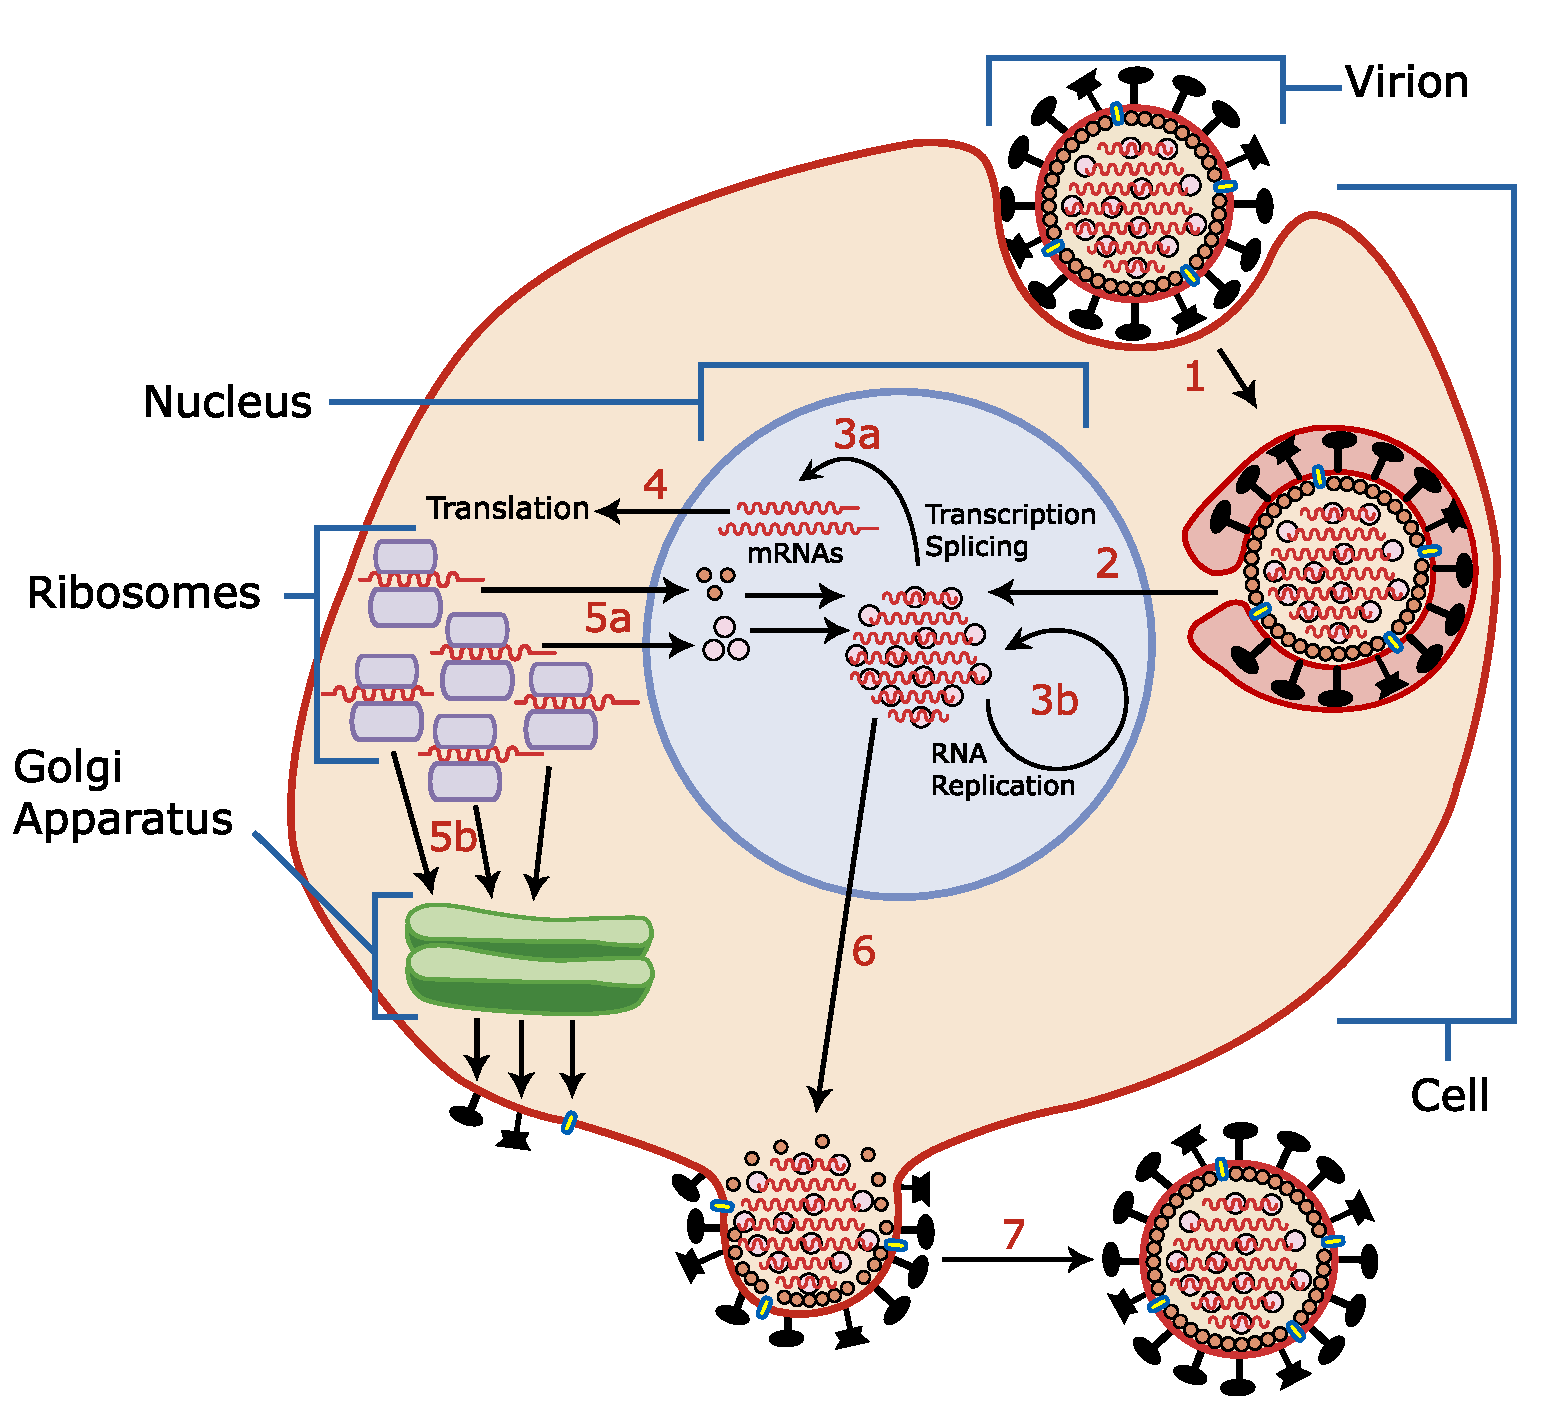
\includegraphics[width=0.6\linewidth]{Figures/Virus_Replication_large.pdf}
    \caption{The life cycle of a virus begins with a virion (virus particle) being absorbed by the cell. Once the virion enters into a cell the virus genome is released. The genome moves to the ribosomes, where the genome is replicated. With the replicated genome, new virus can be assembled by the golgi apparatus and then released from the cell.}
    \label{fig:Virus_Replication}
\end{figure}

Some viruses cause illnesses and a few of them are severe enough to receive global recognition: the 2019-2020 coronavirus pandemic (a widespread global outbreak), the 2014 outbreak of Ebola in West Africa, and the 2009 H1N1/swine flu pandemic, for example. Another virus that has become well known is influenza (or the flu). In total, the Centers for Disease Control and Prevention (CDC) estimates that in the United States up to 42.9 million people were sick during the 2018-2019 flu season, 647,000 people were hospitalized, and 61,200 died \cite{website4}.

In order to understand viruses, assays are performed. An assay is an experiment for assessing or measuring characteristics of a substance. The two typical forms of assays are quantitative and quantal. Quantitative assays are assays that give an accurate and exact measure of the amount of a substance in a sample. Of these types of assays, plaque assays are the most widely used for determining viral titer \cite{Kumar}. They can be used with any virus that causes damage to the cells where they have been grown. This damage is called a plaque and is circular in shape. These assays are often performed in petri dishes, where virus is placed in a dish of healthy cells and the formation of plaques and the concentration of virus are monitored. It is assumed that each plaque formed is caused by one virus particle. Because of this assumption, the viral concentration is often recorded as plaque forming units per milliliter (pfu/mL). Quantal assays are assays which generally give only a pass or fail. These assays are performed in many mediums such as in animals or in multi-well plates. Any virus that will infect the medium can be used. When multi-well plates are used, different groups of wells on the plate are filled with a dilution of virus that often varies in a ten fold difference from group to group. After a set amount of time the wells are observed for a reaction, and whether or not a well has a response is counted. When animals are used, different animal subjects are injected with a dilution of virus that often varies in a ten fold difference from subject to subject. After a set amount of time the animals are observed, and whether or not an animal dies is counted.

\subsection{Viral Transmission}
\todo[noline, color=red!40]{Once you find some papers here, you can expand this by discussing specific findings from the papers.}

A major determinant of infection progression is how viruses are transmitted through the body. This transmission occurs by two modes: cell free transmission and cell to cell transmission. A viruses can transmit by an individual mode or both modes. During cell to cell transmission, some virus spreads to a neighboring cell through an inter-cellular transfer, as seen in figure \ref{fig:cell2cell}. During cell free transmission, cells release virus that diffuses throughout the body and can cause any cell that the virus enters to become infected.

\begin{figure}[h]
    \centering
    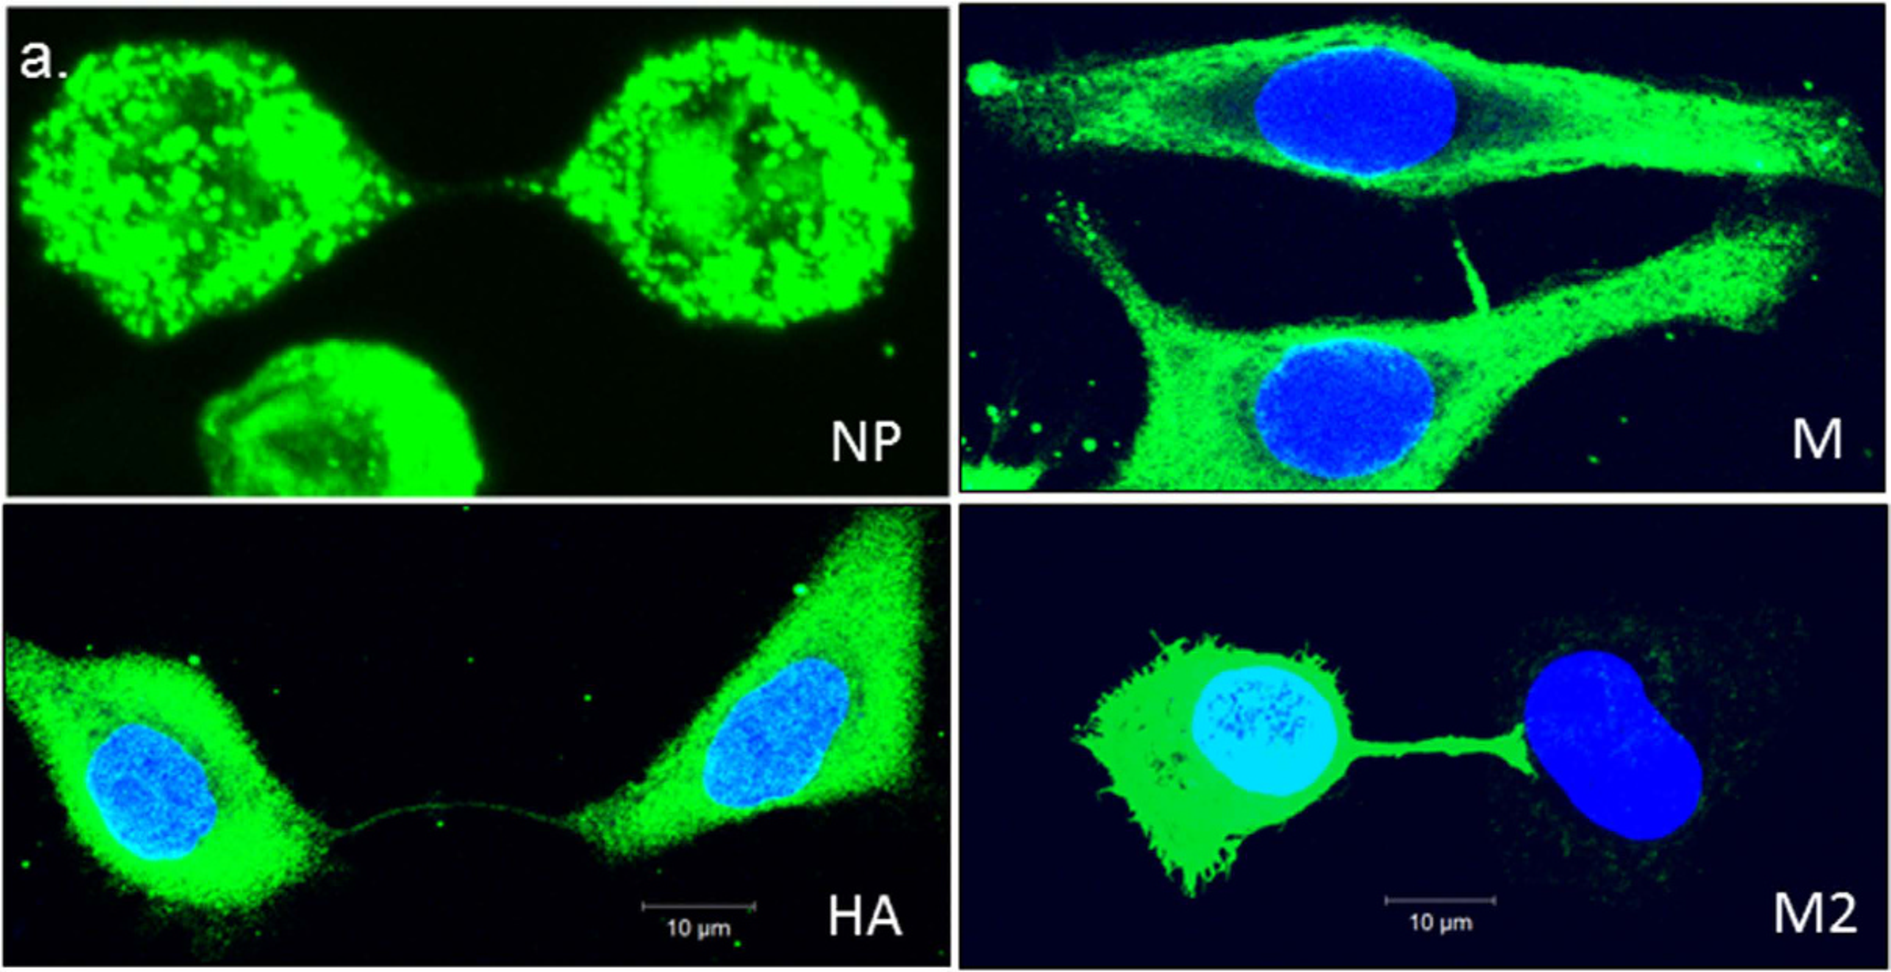
\includegraphics[width=0.8\linewidth]{Figures/cell2cell.pdf}
    \caption{Some virus spread to neighboring cells through an inter-cellular transfer. Tunneling nanotubes (TNTs) serve as a conduit for this transfer. The fluorescent images show influenza virus proteins within TNTs. As mentioned in \cite{cell2cell}, the viral proteins are labeled with anti-tubulin antibodies and anti-mouse antibodies conjugated to Alexa Fluor 488 and the cells are stained with Alexa594-Phalloidin and DAPI.}
    \label{fig:cell2cell}
\end{figure}

Most viruses do not transmit by the two modes equally, which results in different dynamics for each viral infection. A characteristic of cell to cell transmission is that if a virus is transferred, the virus is protected from the extracellular fluid. This means that the immune system and antiviral drugs that are in the body/extracellular fluid will not interact with the virus and therefore have no effect \cite{Allen}. Previous research has used mathematical models to investigate the effects of cell to cell transmission, using ordinary differential equation models \cite{Allen, Wang, Pourbashash} and a stochastic model \cite{Allen}. However, these studies do not account for how infection spread is affected by the spatial aspect of cell to cell transmission. If the spatial structure in an infection is ignored, this can lead to biased or incorrect estimates of parameter values and to qualitatively different behavior from what is actually occurring during the infection \cite{Gallagher}. This work will include two dimensional geometry, to allow for the spatial aspect, in the investigation of cell to cell transmission.

Along with the different transmission modes there are other aspects of viruses that can affect how a virus transmits through a body. Many viruses, such as herpes simplex virus (HSV-1), human immunodeficiency virus (HIV), mink enteritis virus (MeV), and respiratory syncytial virus (RSV), cause cells to fuse together into large multi-nuclear cells known as syncytia \cite{Carmichael, Chowdhury, Rozieres, Tian}. The virus enables this fusion, so each syncytium is already infected and will produce virus. These syncytia have a role in the dynamics of viral infection, but the specifics of what the syncytia do is not well understood. There are currently no published models on how syncytia formation affects infection. This work will aim at characterizing parameters of syncytia, such as production rate and lifespan, to gain insight. The amount of virus that is produced is unknown; it could be more or less than the unfused cells. It is also unknown if the syncytia have longer or shorter lifespans than the unfused cells. This could lead to several different outcomes in the viral infection, as seen in table \ref{tab:SyncytiaProduction}.

\begin{table}[h]
    \centering
    \caption{Potential outcomes of viral infection caused by Syncytia.}
    \begin{tabular}{|c|c|c|}
        \hline
          & Produces More Virus & Produces Less Virus\\
        \hline
        Longer Life Span & More Severe Infection & Unknown difference in Severity\\
        \hline
        Shorter Life Span & Unknown difference in Severity & Less Severe Infection\\
        \hline
    \end{tabular}
    \label{tab:SyncytiaProduction}
\end{table}

Aside from a virus's inherent properties, there are phenomena in the host's body that can affect viral transmission as well. When influenza virus enters the human respiratory tract, the virus enters in through the upper respiratory tract, as seen in figure \ref{fig:RespiratoryTract}. There, the virus diffuses through the mucus that coats the air ways and can migrate down to the lower respiratory tract. A flow of the mucus (advection) upwards away from the lower respiratory tract, caused by cilia on some of the cells pushing the mucus upwards, can slow or prevent the virus from spreading. A variation in speed of the mucus flow can change the result of each infection, especially since the speed depends on the age and health of the host.

\begin{figure}[H]
    \centering
    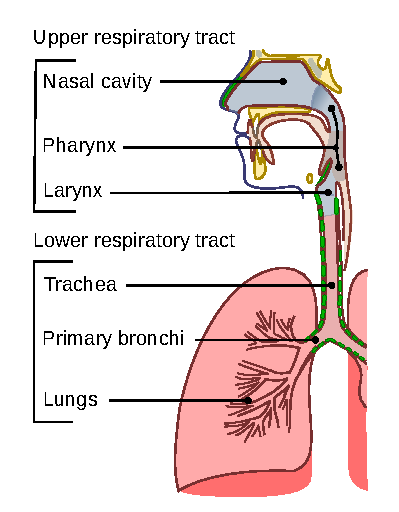
\includegraphics[width=0.4\linewidth]{Figures/Illu_conducting_passages.pdf}
    \caption{The respiratory system has two main tracts, the upper and lower. Virus can enter into the upper respiratory tract and migrate down to the lower respiratory tract. Once the virus is in the lower respiratory tract worse infections, such as pneumonia and bronchitis, can occur.}
    \label{fig:RespiratoryTract}
\end{figure}

\noindent
Viral infections in the respiratory tract can be substantial causing death and hospitalization in infants \cite{Geoghegan} and the elderly \cite{Fleming}, yet only causing mild infections in healthy adults \cite{Hall, Lee, Bagga, Mills}. Small children and the elderly happen to have lower mucus velocities than adults \cite{Sturm, Puchelle, Grubb, Oliveira, Ho}; this decrease in upward advection may allow virus to diffuse down and into the lower respiratory tract. Infections in the lower respiratory tract tend to be more severe \cite{Naorat, Kaneko, Shi, Atwell, HallC, Takeyama, Park}, causing conditions such as pneumonia and bronchitis. Mathematical models have been used to investigate advection in the human respiratory tract in order to gain insight on how it changes the viral infection. Two of the models are a one dimensional partial differential equation model \cite{Quirouette} and an ordinary differential equation model \cite{diffusionmodel}. The prior models either did not account for or had a very simple extension of the spatial aspect of a infection in the respiratory tract. Both models concluded that there is a threshold of advection that does not allow the virus to move down the respiratory tract. Gonzalez-Parra et al. \cite{diffusionmodel} concludes that the advection threshold speed depends on infection parameters (like those in Table \ref{tab:parameters}). However, Quirouette et al. \cite{Quirouette} concludes that the location of initial infection within the respiratory tract determines spread of the infection to the lower respiratory tract. Their work showed that virus did not spread down the respiratory tract, in the presence of advection, from where the initial infection occurred. This work will develop a more realistic model of the respiratory tract in order to investigate advection further.\\

The full effects that each of these different phenomena has on viral spread is unclear. For a particular virus, an understanding of how viral infections are affected by the rate at which a virus will transmit cell to cell, the formation of syncytia, and the speed of the mucus flow in the respiratory tract (advection) is required in order to administer the correct drugs to patients. This work aims to characterize the role of different phenomena, which will result in better understanding in lab studies.

\subsection{Choice in model vs. experiment}
The use of assays is crucial to studying viruses, but they do have some limitations. Performing many assays requires a lot of funds, labor, and time to make the different measurements for analysis. This leads to either data not being collected as often as might be necessary or not enough cases being studied to capture all of the fine details of an infection. Another difficulty with assays is that some characteristics of viruses cannot be controlled for in experiments. For example, it's difficult to stop all of the cell to cell transmission or all of the cell free transmission. This makes it impossible to have an isolated study of one characteristic of an infection. By using computer models, many cases with more frequent data collection can be performed using fewer resources.

\section{Approach/Methodology}
%\textcolor{blue}{
%How are you going to do the study? Are the overall strategy,
%methodology, and analyses well-reasoned and appropriate to accomplish the specific aims of the project? Have the investigators presented strategies to ensure a robust and unbiased approach, as appropriate for the work proposed? Are potential problems, alternative strategies, and benchmarks for success presented?}
%\\

The system that will be simulated is a culture dish where there is a two dimensional layer of cells with virus diffusing over the cells. The simulation will be a hybrid of an agent based model (ABM) and a partial differential equation model (PDEM) where the cells will be simulated with an ABM and the virus diffusion will be simulated by a PDEM.
\\

In a PDEM, the dynamics of a system can be represented by a partial differential equation or more specifically, an equation that contains multi-variable functions that represent important system aspects and one or more partial derivatives of those functions. In the culture dish, as an infected cell releases virus into the extra cellular fluid, the virus will diffuse across a density gradient. With the PDEM, diffusion will be represented by the diffusion equation, 

$$\frac{\partial V}{\partial t}=D \nabla^{2}V,$$

\noindent
where $V$ is the density of the virus and $D$ the diffusion matrix. This diffusion is a crucial aspect of one of the modes of viral transmission studied in this paper and therefore the simulation would be incomplete without it.

An ABM breaks a system down into smaller units, or agents, and each agent is governed by a set of rules. As the simulation is stepped through time, the agents act and interact.  These actions cause bulk properties, at the system level of the simulation, to become apparent for observation and measurement. In any culture dish \cite{website1} there is on the order of $10^6$ cells. With the ABM there will be on the order of $10^6$ agents made, this will allow for the simulation to reproduce what is happening in the dish. The ability to manipulate what is happening at the cellular level of the simulation will allow for generation of isolated studies of single viral transmission modes and combinations of viral transmission modes. These isolated studies of how cells are infected, will be analyzed for the characteristics discussed at the end of this section.

For an ABM in a 2-D plane, the minimum number of calculations per time step is on the order of the number of agents times the log base ten of the number of agents, 

$$\mathcal{O}(n\log_{10} (n)).$$

\noindent
So for this system the minimum number of calculations is $6*10^6$. As the model becomes more complex and the calculations increase, parallel processing will be utilized to speed up the simulation run time. ABM's often have an inherent structure that allows the models to be parallelized very simply. A code written in the programming language CUDA can run in parallel on Nvidia brand GPUs. This will allow for simulations to be run on a desktop computer with greater speeds than most clusters.

\todo[inline, color=red!40]{Can you make a graph of \# of agents vs. speed? For cell2cell and cell free? That can probably be used in the comp. sci. paper as well.}%
This work will be completed in two main stages. In the first stage a base code will be created and in the second stage the code will be modified to include other biological processes.

\subsection{Stage one: Completing base code}
The base code will simulate cells that can go through the different stages of infection and properly model how virus can diffuse through a medium above the cells. The ABM will govern the transitions a cell makes through the stages of infection: healthy, eclipse, infected, and dead. A cell in the healthy state is an uninfected cell that remains healthy until infected. A cell in the eclipse state is an infected cell that is not yet producing virus. The cell will remain in the eclipse state until an amount of time that is pulled from a gamma distribution \todo{Be ready to explain why gamma distributions in the exam.} with shape value $\tau_E$ and scale value $\tau_E/\sqrt{\eta_E}$, has passed. A cell in the infected state is a cell that has become infected and has begun to produce virus. The cell will remain in the infected state until an amount of time, that is pulled from a gamma distribution with shape value $\tau_I$ and scale value $\tau_I/\sqrt{\eta_I}$, has passed. A cell in the dead state is a cell that can no longer change state, therefore once a cell is in the dead state the cell will remain in that state until the end of the simulation. The flow of this is illustrated in figure \ref{fig:stages_of_infection}. \todo{Be ready to explain why no cell regeneration in the exam.}

\begin{figure}[h]
    \centering
    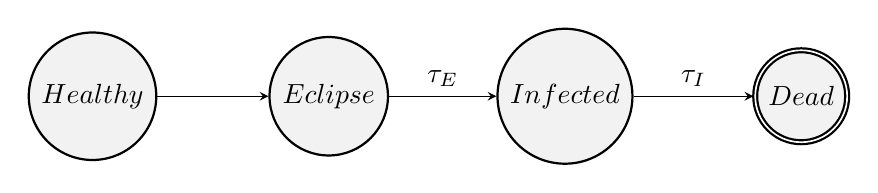
\begin{tikzpicture}
        \node[state] (H) {$Healthy$};
        \node[state, right of=H] (E) {$Eclipse$};
        \node[state, right of=E] (I) {$Infected$};
        \node[state, accepting, right of=I] (D) {$Dead$};
        
        \draw   (H) edge[above] node{} (E)
                (E) edge[above] node{$\tau_E$} (I)
                (I) edge[above] node{$\tau_I$} (D);
    \end{tikzpicture}
    \caption{The stages of infection healthy, eclipse, infected, and dead are shown. Cells stay in  the eclipse stage for an average time $\tau_E$ and in the infected stage for an average time $\tau_I$.}
    \label{fig:stages_of_infection}
\end{figure}

To apply the ABM computationally, four arrays with an element for each cell will be created: universal time (UT), healthy time (HT), eclipse time (ET), and infected time (IT). The universal time array holds the amount of time that each cell has been in the simulation, each element starts at zero and increases each iteration by the simulation's time step. The healthy time array holds the amount of time that a cell is healthy, each element for a healthy cell starts at zero and increases each iteration by the simulation's time step. The eclipse time array will hold the amount of time each cell will be in the eclipse state. Each element in the array is initially filled with a different number pulled from the gamma distribution with shape value $\tau_E$ and scale value $\tau_E/\sqrt{\eta_E}$. The infected time array will hold the amount of time each cell will be in the infected state. Each element in the array is initially filled with a different number pulled from the gamma distribution with shape value $\tau_I$ and scale value $\tau_I/\sqrt{\eta_I}$. The flow of this is illustrated in figure \ref{fig:transitioning_through_the_stages_of_infection}. Through tracking these ``Time" arrays the ABM can transition cells to different states after infection.

\begin{figure}[h]
    \centering
    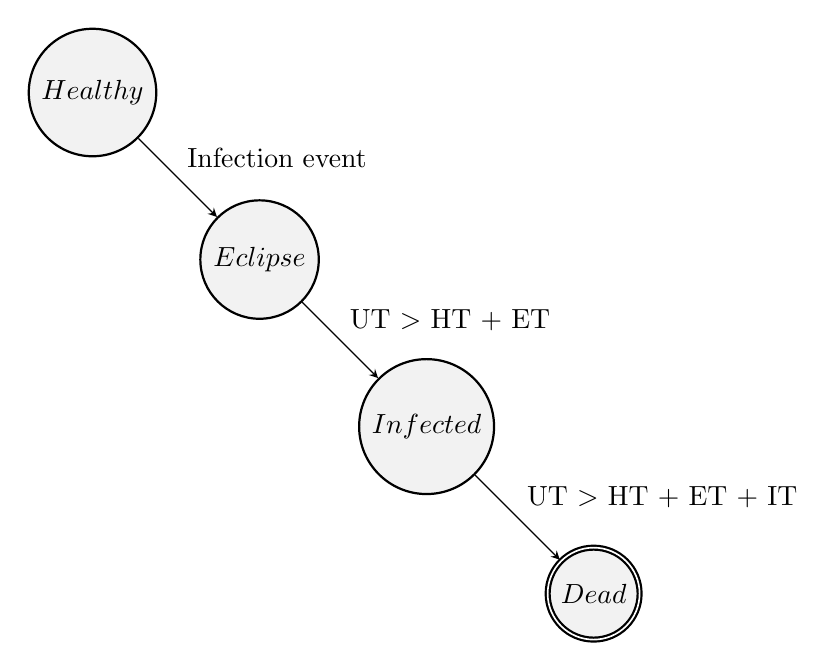
\begin{tikzpicture}
%        \node[state, initial] (H) {$Healthy$}; %Adds arrow at beginning state
        \node[state] (H) {$Healthy$};
        \node[state, below right of=H] (E) {$Eclipse$};
        \node[state, below right of=E] (I) {$Infected$};
        \node[state, accepting, below right of=I] (D) {$Dead$};
        
        \draw   (H) edge[above right] node{Infection event} (E)
                (E) edge[above right] node{UT $>$ HT + ET} (I)
                (I) edge[above right] node{UT $>$ HT + ET + IT} (D);
    \end{tikzpicture}
    \caption{Transitioning through the stages of infection: UT is the universal time for a cell, HT is the healthy time for a cell, ET is the eclipse time for a cell, and IT is the infected time for a cell.}
    \label{fig:transitioning_through_the_stages_of_infection}
\end{figure}

Now to incorporate when a cell becomes infected, we must consider the spatial aspect of the environment the cell is in. In this study a dish or 2-D circular plane of cells has been chosen to be simulated. The dish in which the cells are grown will be assumed to have been grown to confluence, or to the point where the surface of the dish is completely covered by cells, as seen in figure \ref{fig:HexagonalCells}. Figure \ref{fig:A2} shows cells that are stained with Alexa Fluor 488. The stain binds to the zonula occudens-1 (ZO-1), in green, where it is found in the cell to cell connections.
\todo{You should also explain what stain was used to make the A2 image.}%

\begin{figure}[h]
    \centering
    \begin{subfigure}[b]{0.4\linewidth}
        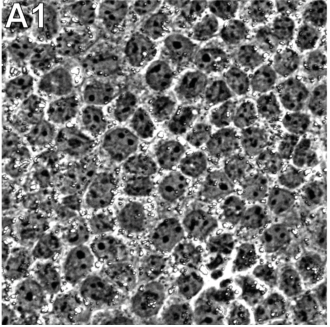
\includegraphics[width=0.8\linewidth]{Figures/CellPhotoA1.pdf}
        \caption{}
        \label{fig:A1}
    \end{subfigure}
    \begin{subfigure}[b]{0.4\linewidth}
        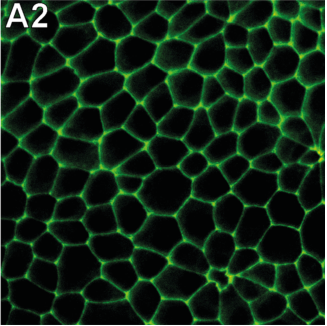
\includegraphics[width=0.8\linewidth]{Figures/CellPhotoA2.pdf}
        \caption{}
        \label{fig:A2}
    \end{subfigure}
    \caption{Confluent Madin-Darby Canine Kidney cells (MDCK II) stained with Alexa Fluor 488. The stain binds to the ZO-1 where it is located in the uppermost cell-cell connection, the tight junctions, at the lateral cell membrane of polarised epithelia. They form a physical barrier to control the lateral flux of ions, macromolecules, pathogens, and other solutes within the paracellular pathway. (a): A contrast image. (b): Fluorescence image for zonula occudens-1 (ZO-1)}
    \label{fig:HexagonalCells}
\end{figure}

The best representation for confluence is for the cells to be represented as hexagons on a hexagonal spatial grid, because the cells are squashed in by their nearest 6 neighbors. Changing to a hexagonal grid means that cartesian coordinates can not be directly used, nor are they the best choice, for calculations in these simulations. This change of coordinate system will not affect the ABM aspect of the code, but it will allow for the ability to determine which cells are adjacent to a cell in question. 

In order for the hexagonal grid to be incorporated into the ABM, there must be a way to identify and index through each of the hexagons. There are different conventions that can be followed to make a grid of hexagons, one way is cube coordinates. In cube coordinates there are three numbers $X_{hex}$, $Y_{hex}$, and $Z_{hex}$ that are used to identify a hexagon. Often people are familiar with cube coordinates if they want to plot hexagons on a x, y plot, because the conversion to 2-D cartesian coordinates from hexagonal coordinates is straight forward. $$x = X_{hex}$$ and $$y = 2/3*\sin(\pi/3)*\left ( Y_{hex}-Z_{hex} \right )$$ There are three other attributes to cube coordinates that are great for making grids:
\begin{enumerate} 
    \item The coordinates can be split in to three sectors where the coordinates $X_{hex}$, $Y_{hex}$, and $Z_{hex}$ are simply cyclic permutations.
    \item The $X_{hex}$ and $Z_{hex}$ coordinates, also known as axial coordinates, can be used as indices of a matrix.
    \item  The coordinates of the neighboring hexagons are found by adding a cyclic permutation of 
        $\left [
            \begin{array}{c}
                1 \\
                0 \\
                -1\\
            \end{array}
        \right ]$
        for three of the neighbors and
        $\left [ 
            \begin{array}{c}
                1 \\
                -1 \\
                0\\
            \end{array}
        \right ]$
        for the other three neighbors.
\end{enumerate}
Attribute 1 allows for quick construction of grids, by reducing the number of hexagon locations to be calculated by a third. Attribute 2 and 3 give the ability to store the hexagon locations in a matrix allowing for simple referencing of the hexagons and their neighbors in a computer code. 

Now that each hexagon and its neighbors can be referenced easily, cases in the code can be built for infection. If infection were to be caused by an adjacent cell the code can now account for it appropriately. This simple referencing also gives the necessary structure to incorporate the diffusion of virus over the cells. In the code, along with the assumption of hexagonal cells, the cells will be assumed to be flat, so the virus is diffusing over a smooth 2-D plane. This assumption will allow for the use of the 2-D diffusion equation, the only change will be that the equation will need to be in hexagonal coordinates. 

$$\frac{\partial V}{\partial t} = D\nabla^{2}V$$

\noindent
becomes 

$$\frac{\partial V}{\partial t} = D\frac{2}{3} \left (\frac{\partial^2}{\partial x^2_1}+\frac{\partial^2}{\partial x^2_2}+\frac{\partial^2}{\partial x^2_3}\right )V$$ 

\noindent
where $x_i$ are the unit vectors for a hexagonal grid, 
$\textbf{x}_1=
\left [
    \begin{array}{c}
        1 \\
        0 \\
    \end{array}
\right ]$, 
$\textbf{x}_2=
\left [
    \begin{array}{c}
        -1/2 \\
        \sqrt{3}/2 \\
    \end{array}
\right ]$, 
$\textbf{x}_3=
\left [
    \begin{array}{c}
        -1/2 \\
        -\sqrt{3}/2 \\
    \end{array}
\right ]$.

\noindent
Now that diffusion of virus has been added to the code, the model can appropriately account for an infection that is caused by the virus diffusing over the cells.
\\

The base code is complete and able to transition cells through the stages of infection, properly modeling the diffusion of virus, and allowing for different modes of transmission to be implemented. In order to analyze what is happening in the simulations, viral titer curves, shown in Figure \ref{fig:VirusVsTime}, will be produced and features of the curves, depicted in Figure \ref{fig:Graphs}, will be measured.
\begin{itemize}
    \item \textbf{peak viral load}: The maximum amount of virus is commonly used as an indicator of the transmissibility of an infection (Handel et al., 2009).
    \item \textbf{time of viral peak}: This is the time between the start of the infection and the peak of the virus.
    \item \textbf{viral upslope}: Viral upslope is the exponential growth rate of the viral titer during the first ∼1 d of infection.
    \item \textbf{viral downslope}: The viral downslope is the exponential decay rate of the viral titer and for ordinary differential equation models is linked to both the lifespan of infectious cells and the clearance rate of virus (Smith et al., 2010).
%    \item \textbf{area under the curve (AUC)}: AUC is often used to assess the severity of an infection (Barroso et al., 2005, Hayden et al., 2000).
%    \item \textbf{infection duration}: The infection duration is defined as the duration of time the viral titer is over $10^{4}$ and is indicative of how long an infected patient might experience symptoms (Dobrovolny et al., 2010). \todo[inline, color=red!40]{In that paper, we used the symptomatic duration which is a $10^4$ threshold. $10^1$ is a typical experimental limit of detection and gives the infection duration.}%
\end{itemize}

\subsection{Stage two: Incorporating different modes of viral transmission}
Virus transmission is affected by four main phenomena: cell to cell transmission, cell free transmission, syncytium formation, and advection. These phenomena are four distinct ways that viruses are transmitted and by looking closely at each transmission mode we get a better and broader understanding of how virus transmission affects the duration and severity of the illness. These transmission modes can be hard to study directly in a lab, so computer models allow for theoretical testing to develop better methods for measuring their effects in the lab.

\subsubsection{Case 1: cell to cell transmission and cell free transmission}
In the simulations both transmission modes (cell to cell and cell free) will be present, but the probability of infection for cell to cell transmission will be varied. The probability ($\mathrm{P_{c2c}}$) that a cell will become infected, via cell to cell transmission, is predefined,

$$\mathrm{P_{c2c}} = \{x \in \mathbb{R} \mid 0<x<1\}.$$

\noindent
When a healthy cell has an infected neighbor a number is pulled from the uniform distribution and is compared to the probability. If that number is less than the probability, then the cell will become infected. The probability does not change if a cell has multiple infected neighbors, because the check for infection occurs for each infected neighbor, therefore naturally increasing the probability. For cell free transmission the probability ($\mathrm{P_{cf}}$) that a cell will become infected is defined by the amount of virus that is covering the cell (V) times the infection rate ($\beta$) times the time step of the simulation ($\Delta t$) \cite{Holder}.

$$\mathrm{P_{cf}} = V \beta \Delta t$$ 

\noindent
As a healthy cell becomes covered in virus the probability of cell free infection increases. If the probability ($V \beta \Delta t$) is ever greater than one due to the build up of virus, an adaptive time step is used. The time step ($\Delta t$) is divided in half repeatedly, until the probability is below one. Once the probability is finalized, a number is pulled from the uniform distribution and compared with the probability. If that number is less than the probability, then the cell will become infected.

The measurements (from ``Stage one": peak viral load, time of viral peak, viral upslope, and viral downslope) will be plotted against the fraction of cells infected via cell to cell transmission. These could show a relationship that can be used to calibrate the measurements done in a lab allowing experimental determination of the fraction of cells infected via each transmission mode.

\subsubsection{Case 2: Syncytia Formation}
In the simulations, syncytia can form when two infected cells are adjacent to one another and when an infected cell is adjacent to a syncytium. The formation of syncytia happen with a probability ($\mathrm{P_{s}}$),

$$\mathrm{P_{s}} = \{\gamma \in \mathbb{R} \mid 0<\gamma<1\}.$$

\noindent
During syncytium formation, if transmission is successful, a number is pulled from the uniform distribution and compared to the probability. If the number is less than the probability, then a syncytium is formed. If an infected cell is adjacent to another infected cell or syncytium, then a number is pulled from the uniform distribution and compared to the probability. If the number is less than the probability, then the infected cell is added to the syncytium.

The measurements (from "Stage one": peak viral load, time of viral peak, viral upslope, and viral downslope) will be plotted against syncytia production rate ($\rho _s$) and syncytia lifespan ($1/\delta _s$). These could show a relationship that can be used to calibrate the measurements done in a lab for syncytia formation and help determine if syncytia production rate and syncytia lifespan can be experimentally measured.

\subsubsection{Case 3: Advection}
In order to study advection, the model will be modified from a two dimensional plane to an open cylinder. This cylinder will represent the respiratory tract, where the cells are on the surface. Without added advection, the virus diffuses via a density gradient over the inner surface of the cylinder. In the simulation, advection will impart directed motion to the diffusing virus along the z axis of the cylinder, to resemble the flow of mucus upwards from the lower respiratory tract to the upper respiratory tract. To include this in the model, a drift term will need to be added to the diffusion equation

$$\frac{\partial V}{\partial t} = D\nabla^{2}V + \mu \frac{\partial}{\partial z},$$ 

\noindent
where $\mu$ is the velocity of the mucus. The magnitude of the advection will be varied to see if a critical speed of advection can be found that does not allow the virus to spread down the respiratory tract. The simulations with advection will be compared to simulations without to see how the infections differ.

\section{Analysis Methods/Assessment}
%\textcolor{blue}{Is the plan for carrying out the proposed activities well-reasoned, well-organized, and based on a sound rationale? Does the plan incorporate a mechanism to assess success? What measurements, comparisons, statistical tests, will be utilized to measure success? What significance level is required to provide a measurably clear answer to the posed scientific question(s)?}

\subsection{Direct Comparison}
The data that is produced from the simulations will be compared with experimental data when possible. Figure \ref{fig:CurveWithBaccamData} displays the viral titer curves from six patients shown in dots. To create the data the six patients were experimentally infected with influenza A/Hong Kong/123/77. The patients were prescreened to ensure that they did not already have an influenza infection. Nasal washes were collected daily for the first week of infection and cultured virus titers were recorded. Figure \ref{fig:CurveWithBaccamData} also shows a scaled line of generated data from the computer model. Note that our model was not specifically calibrated to fit this data, but does a reasonable job capturing the general trends.

\begin{figure}[h]
    \centering
    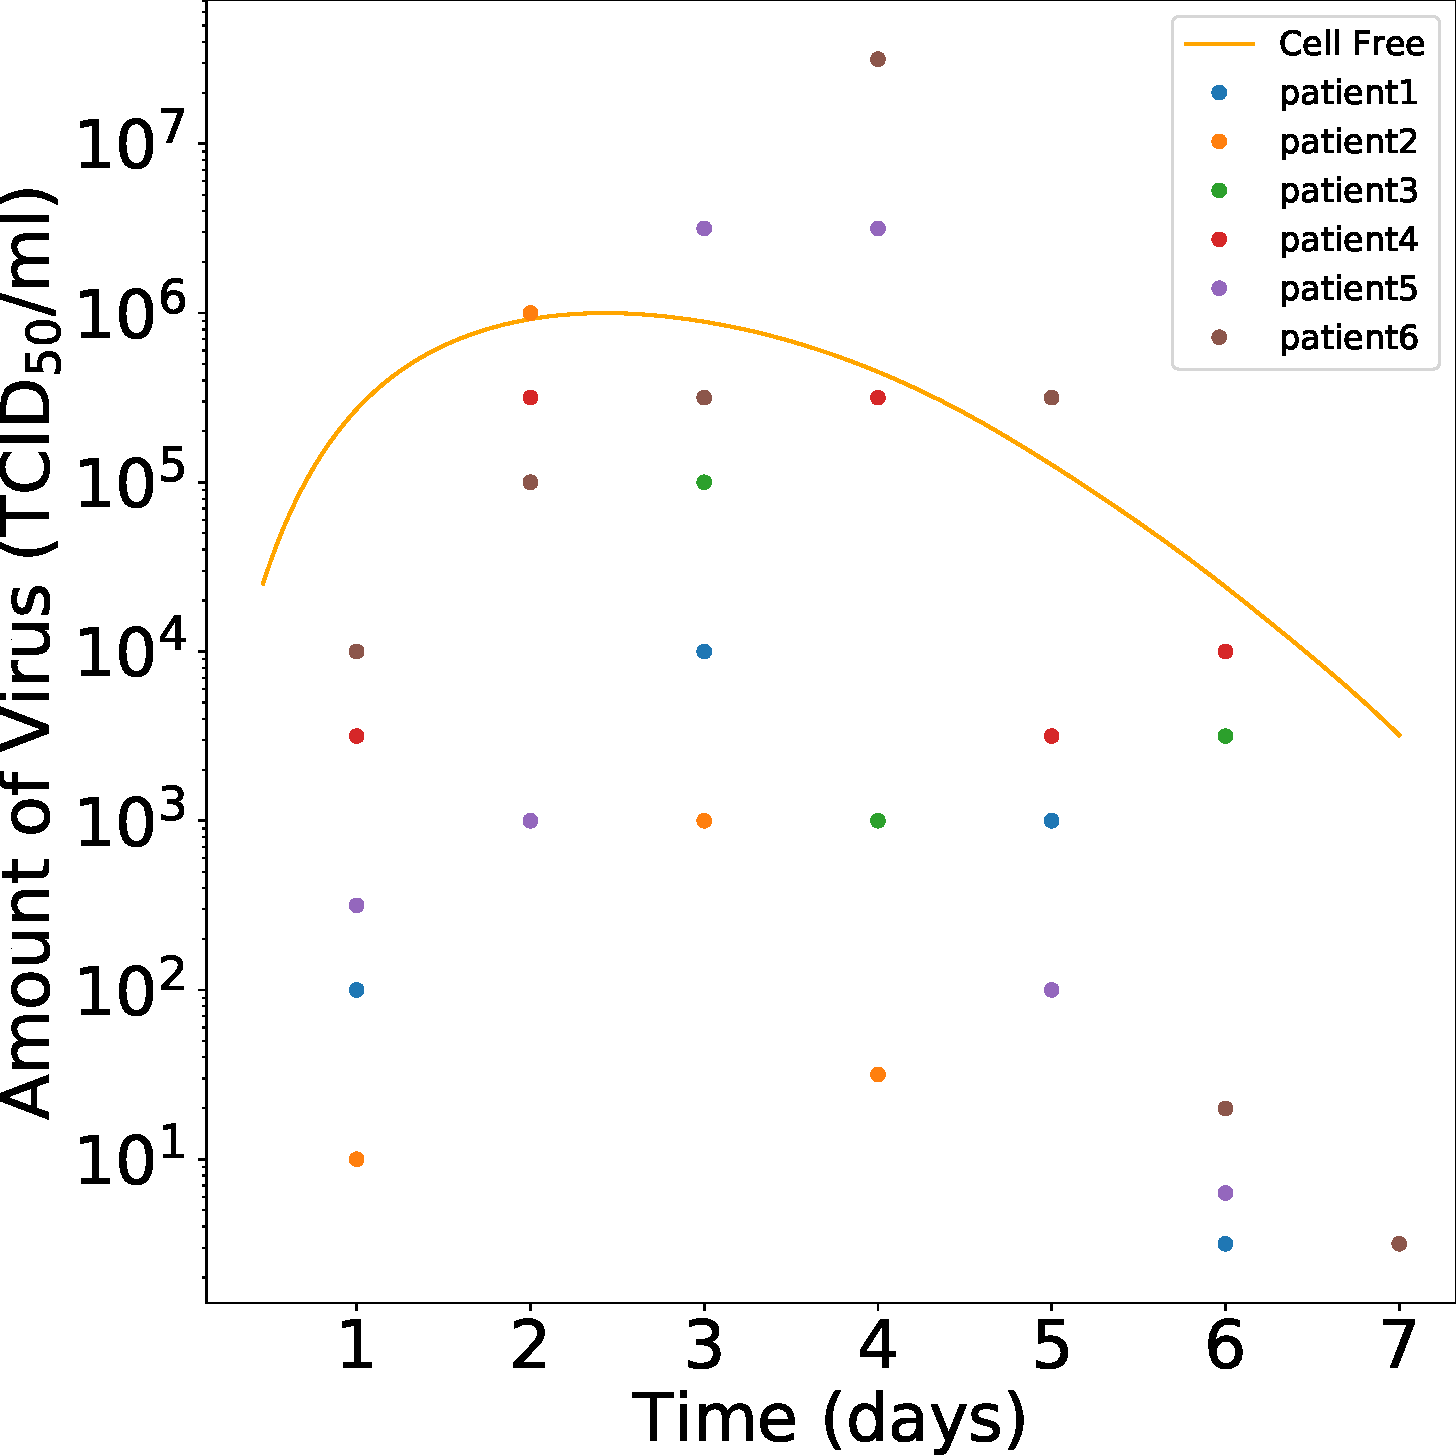
\includegraphics[width=0.6\linewidth]{Figures/MOI_-30_CellToCell_CellFree_ViralTitter.pdf}
    \caption{Viral titer data. (dots) P. Baccam, et al. study, six patients were infected with influenza A/Hong Kong/123/77. Nasal washes were collected daily for the first week of infection and cultured virus titers were recorded. (line) Scaled simulated data from the model with parameters same as those in table \ref{tab:parameters}.}
    \label{fig:CurveWithBaccamData}
\end{figure}

As a visual check the simulated plaque assays will be compared to actual plaque assays. Figure \ref{fig:ActualPlaques} is a petri dish from a plaque assay that infected Madin-Darby Canine Kidney (MDCK) cells with influenza virus A/Memphis/14/96-M (H1N1). The virus was placed in the dish and then after one hour a solution of Avicel RC-581 was injected on to the the cells. The Avicel RC-581 allows for plaques to form by hindering the flow of virus through the liquid medium in the dish. When the experiment was done, the assays were stained with an immuno-stain that stains the infected cells red. Figure \ref{fig:SimulatedPlaques} shows the simulated assay of $10^{6}$ cells, where the green are the healthy cells, cyan are the eclipse cells, red are the infected cells, and black are the dead cells. The plaques appear to be similar between the actual and simulated assays.

\begin{figure}[h]
    \centering
    \begin{subfigure}[b]{0.4\linewidth}
        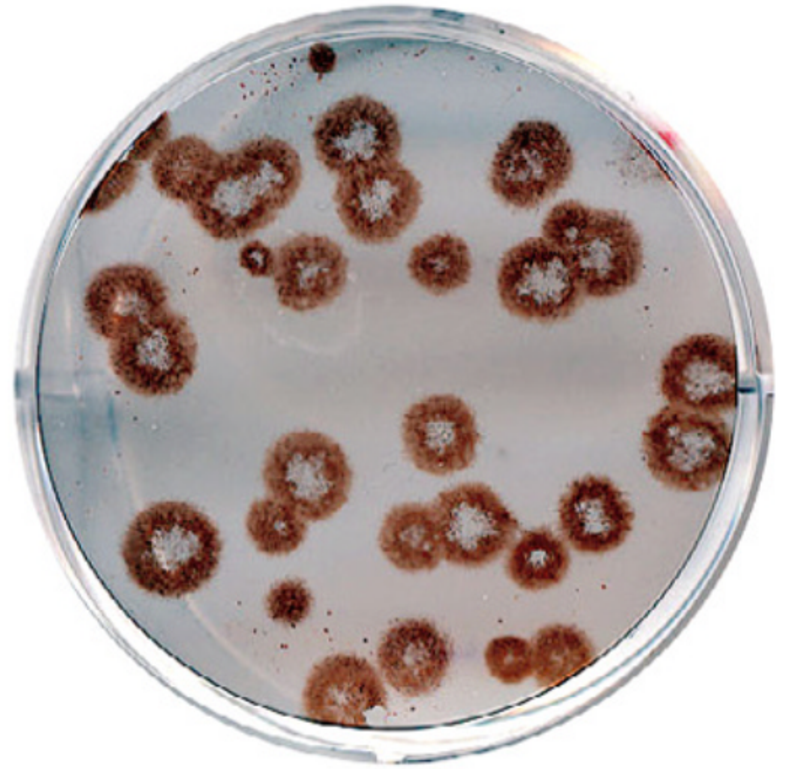
\includegraphics[width=1.0\linewidth]{Figures/plaques.pdf}
        \caption{}
        \label{fig:ActualPlaques}
    \end{subfigure}
    \begin{subfigure}[b]{0.4\linewidth}
        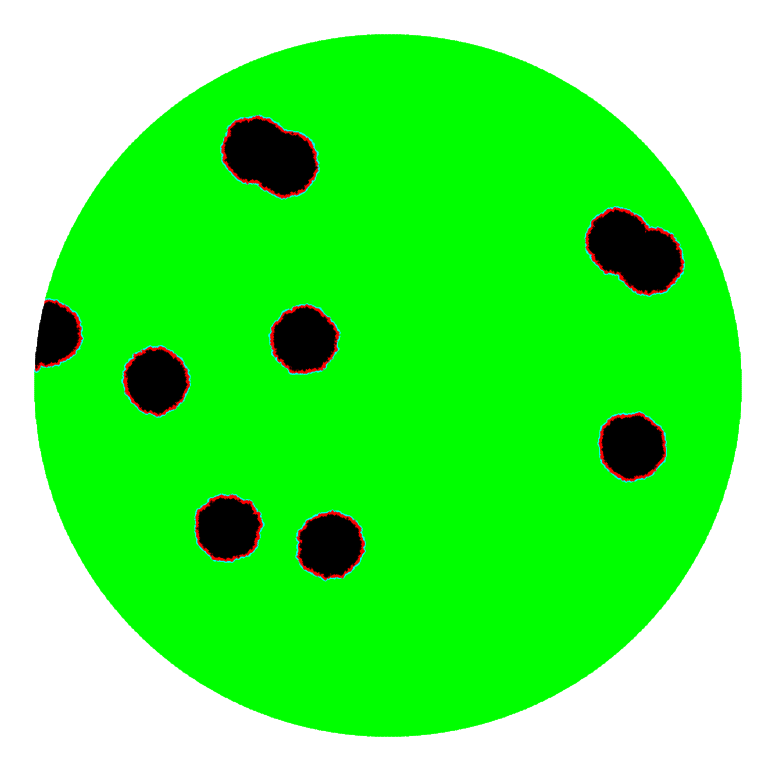
\includegraphics[width=1.0\linewidth]{Figures/cell145.png}
        \caption{}
        \label{fig:SimulatedPlaques}
    \end{subfigure}
    \caption{(Left) Plaque assay that infected Madin-Darby Canine Kidney (MDCK) cells with influenza virus A/Memphis/14/96-M (H1N1). (Right) Simulated plaque assay of $10^{6}$ cells, where the green are the healthy cells, cyan are the eclipse cells, red are the infected cells, and black are the dead cells}
    \label{fig:Plaques}
\end{figure}

Advection speeds have been found for infants/small children \cite{Sturm} and the elderly \cite{Puchelle}, as seen in table \ref{tab:AdvectionSpeeds}. These values will be compared with threshold advection rates generated by the model, in order to gain insight on the higher prevalence of lower respiratory infections in children and the elderly.

\begin{table}[h]
    \centering
    \caption{Advection speeds for different ages.}
    \begin{tabular}{|c|c|}
        \hline
        1 year  & 1.2 mm/min\\
        \hline
        5 year  & 2.7 mm/min\\
        \hline
        adult  & 5.5 mm/min\\
        \hline
        elderly  & 1.3 mm/min\\
        \hline
    \end{tabular}
    \label{tab:AdvectionSpeeds}
\end{table}

\subsection{Statistics}
500 simulations for each transmission mode (cell to cell and cell free) and characteristic (peak viral load, time of viral peak, viral upslope, and viral downslope) of the virus vs time graph will be generated. To determine if the cell to cell and cell free data are statistically independent, the Mann–Whitney U test (U-test) will be used. The U-test is being used instead of the T-test because the T-test assumes that the two distributions (samples) being tested are normal. To test if the data is normal the Shapiro-Wilk, D'Agostino's K-squared, and Anderson-Darling tests will be used. Figure \ref{fig:Hist} shows the distribution of the time of peak virus data that is not normal. Of the distributions in characteristics of virus vs. time graphs generated only the peak amount of virus had a normal distribution in values.

\begin{figure}[h]
    \centering
    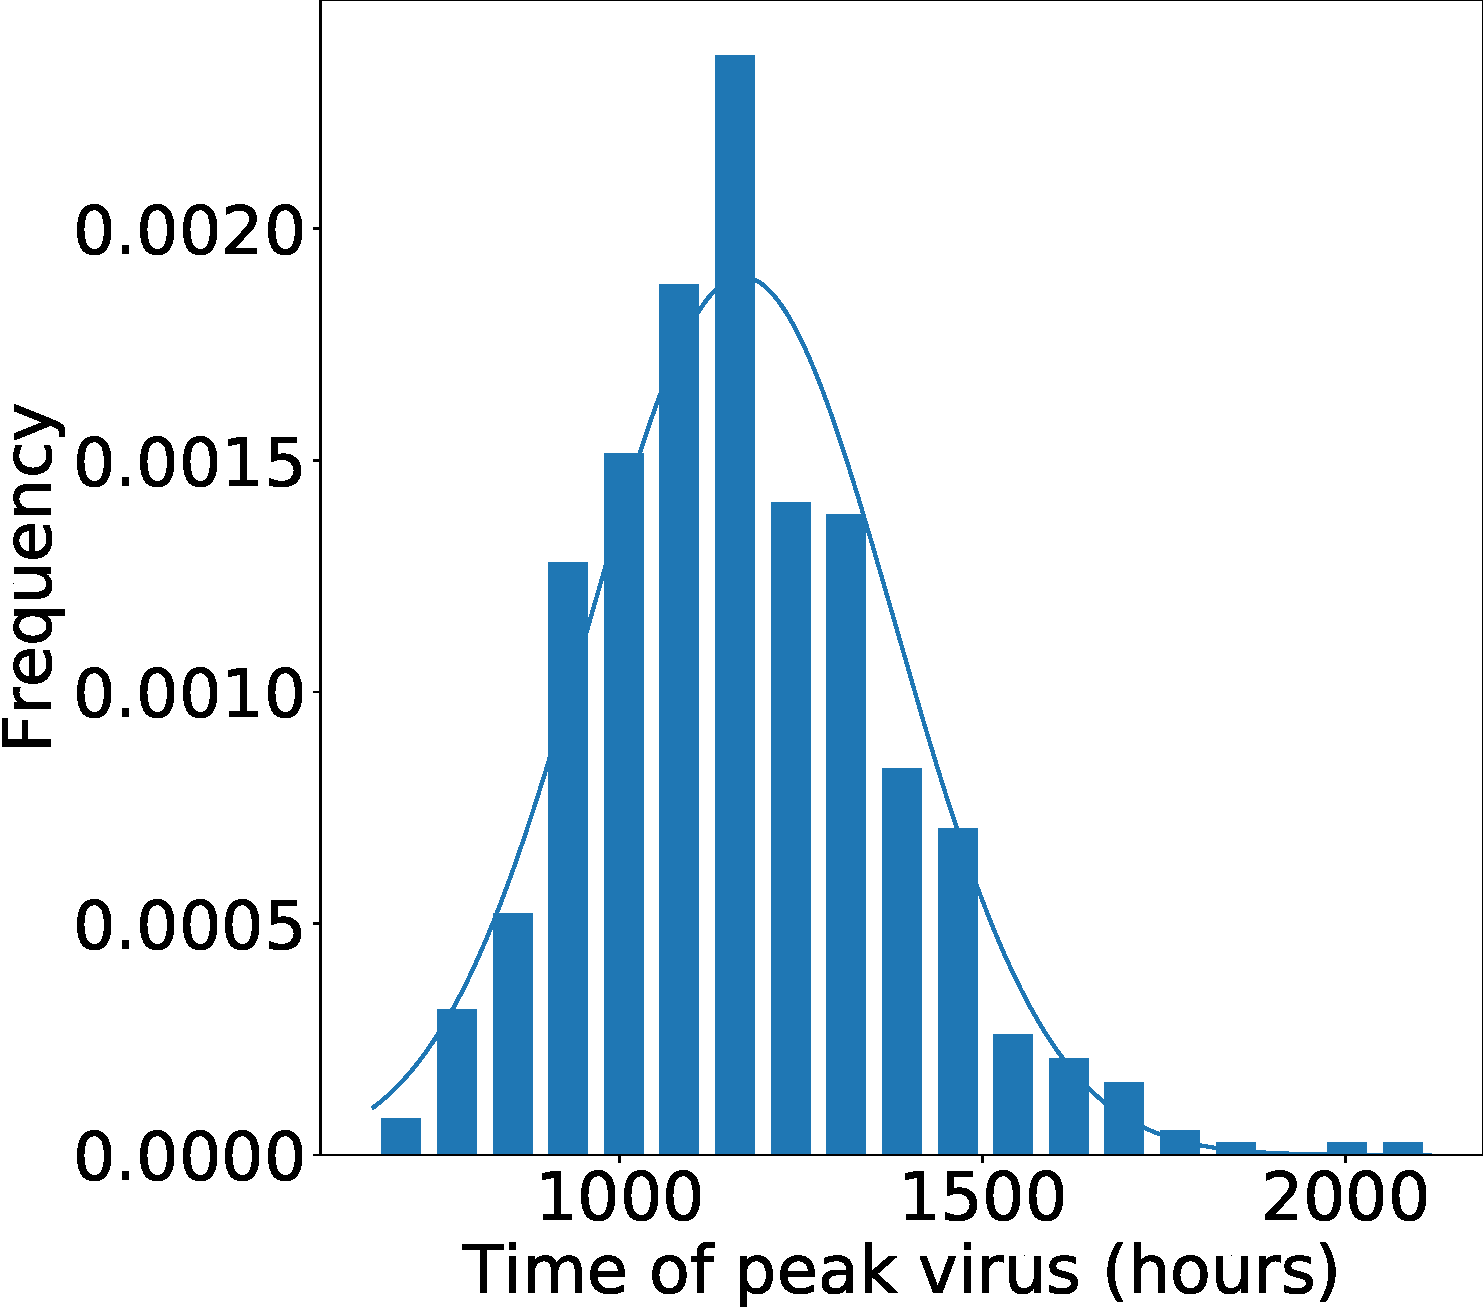
\includegraphics[width=0.45\linewidth]{Figures/-50_TimeOfPeakHist.pdf}
    \caption{A histogram of the time of peak virus measurements from the 500 simulations.  The distribution of the data is not normal. A normal distribution with the same mean and standard deviation is also plotted for comparison.}
    \label{fig:Hist}
\end{figure}

%The simulations can be used to find trends between different aspects of viral dynamics by plotting the average of the 500 simulations, for a given aspect, against an aspect in question. 

We want to use the simulations to help design experiments that can measure aspects of viral dynamics which cannot be measured directly, such as the amount of virus produced by syncytia. Our simulations can be used to find trends between measurable features of the viral titer and these underlying viral dynamics aspects. We will run simulations and plot different experimentally measurable features of the viral titer (listed in section 3) as a function of the aspect we are trying to measure, such as syncytia production rate. If the result of the plotting shows a one-to-one correlation between the measurable features and the underlying aspects, this means that the two properties are directly related. Knowing how the aspects of viral dynamics and the measurable features are related can help in finding a way to measure the aspects in an experiment. For example, if the peak viral titer is measured to increase as the virus production rate by syncytia increases in a one-to-one fashion then an individual performing an experiment could measure the peak viral titer then find the syncytia production rate.

%\clearpage
\section{Research Plan/Timeline/Milestones}
%\textcolor{blue}{Is there specific descriptions of the activities required, there anticipated duration, and a plan in place to document the outputs of those activities? Are there adequate resources available (either at TCU or through collaborations) to carry out the proposed activities?}

\begin{centering}
{\makegapedcells
\begin{longtable}{|p{0.25\textwidth}|p{0.65\textwidth}|}
    \hline
    \raggedleft \Large \textbf{Date} & \Large \textbf{Milestones}\\
    \hline
    \begin{itemize} 
    \raggedleft 
        \item[] Summer 2020
    \end{itemize} 
    &
    \begin{itemize} 
        \item Run simulations with varying cell to cell probability
        \item Submit article on effect of multiplicity of infection
        \item Submit computer science article 
    \end{itemize}\\
    \hline
    \begin{itemize} 
    \raggedleft 
        \item[] Fall 2020 
    \end{itemize}
    & 
    \begin{itemize} 
        \item Compare cell to cell results to experiment, prepare manuscript.
        \item Defend Masters
    \end{itemize}\\
    \hline
    \begin{itemize}
    \raggedleft 
        \item[] Spring/Summer 2021 
    \end{itemize}
    & 
    \begin{itemize} 
        \item Run syncytia formation simulations
        \item Submit cell to cell paper
    \end{itemize}\\
    \hline
    \begin{itemize}
    \raggedleft 
        \item[] Fall 2021 
    \end{itemize}
    & 
    \begin{itemize} 
        \item Prepare and test code with advection
        \item Prepare syncytia manuscript
    \end{itemize}\\
    \hline
    \begin{itemize}
    \raggedleft 
        \item[] Spring 2022
    \end{itemize}
    &
    \begin{itemize} 
        \item Run advection simulations
        \item Submit syncytia manuscript
    \end{itemize}\\
    \hline
    \begin{itemize}
    \raggedleft 
        \item[] Fall 2022
    \end{itemize}
    & 
    \begin{itemize} 
        \item Prepare advection manuscript
        \item Write dissertation
    \end{itemize}\\
    \hline
    \begin{itemize}
    \raggedleft 
        \item[] Spring 2023 
    \end{itemize}
    & 
    \begin{itemize} 
        \item Defend Ph.D
        \item Submit advection manuscript
    \end{itemize}\\
    \hline
\end{longtable}
}
\end{centering}

\section{Progress to date}
%\textcolor{blue}{Has there already been early work on the project (e.g., data collection, etc.)?}

\todo[inline, color=red!40]{You should write this section roughly in the style of a paper --- intro, methods, results, discussion --- but without formally sectioning things off. It will be easier to transfer to a paper that way; it's also how scientists are used to processing information.}%

In a virus study, the inoculum dose is the initial amount of virus used. The different amounts of virus are represented by the multiplicity of infection (MOI). MOI is the ratio of the number of viruses to target cells. This results in a fraction of the number of cells that will be initially infected in a simulation. It is therefore also correlated with the amount of virus that will be produced by infected cells at the beginning of that study. Understanding inoculum dose can lead to a better understanding of key aspects of viral dynamics \cite{Li} (such as cell to cell and cell free transmission) and can help distinguish which aspects are contributing to the dynamics \cite{Moore}. This can in turn help in the production of vaccines \cite{Li}. For severe viruses, like the 2009 H1N1 Influenza pandemic and 2019-2020 Coronavirus pandemic, vaccine development is a race against time. Having a more systematic way, instead of trial and error approach, to determine optimal vaccine protection with a minimal required vaccine dose is necessary. To investigate inoculum dose, a plaque assay model was developed using an agent based model and partial differential equation model. Figure \ref{fig:ZoomedInEclipse} shows a snapshot of the simulated assay. The different stages of infection can be seen: the green are the healthy cells, cyan are the eclipse cells, red are the infected cells, and black are the dead cells.

\todo[inline, color=red!40]{Find some pictures of virus plaques --- you can show that your "plaques" look similar to experiments.}%

\begin{figure}[h]
    \centering
    \begin{subfigure}[b]{0.4\linewidth}
        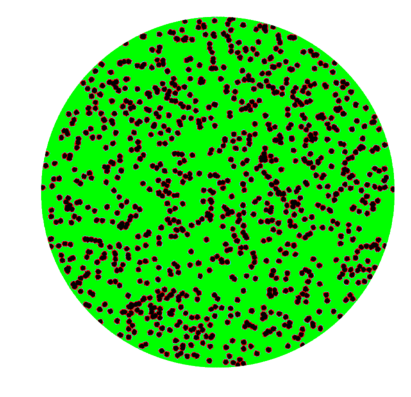
\includegraphics[width=\linewidth]{Figures/EclipseCells.pdf}
        \caption{}
        \label{fig:Dish}
    \end{subfigure}
    \begin{subfigure}[b]{0.4\linewidth}
        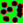
\includegraphics[width=\linewidth]{Figures/ZoomEclipseCells.pdf}
        \caption{}
        \label{fig:ZoomedInEclipse}
    \end{subfigure}
    \caption{(Left) The simulated dish after two simulated days. (Right) A zoomed in section showing all the stages of infection. The green are the healthy cells, cyan are the eclipse cells, red are the infected cells, and black are the dead cells.}
    \label{fig:EclipseCells}
\end{figure}

Virus spreads through a body in two known ways: cell free transmission and cell to cell transmission. Figure \ref{fig:celltocell} shows the first eight days of a simulation with an MOI of $10^{-3}$ with the cell to cell transmission on the left and the cell free transmission on the right. We see that the cell free transmission spreads more quickly than the cell to cell transmission, with most of the cells dying by the eighth day. In order to understand how inoculum dose affects the two transmission modes, the initial amount of virus is varied and total virus over time graphs are generated for the corresponding MOI (initial amount of virus).

\clearpage
\begin{center}
\begin{minipage}{0.65\linewidth}
\begin{figure}[H]
    \centering
    \begin{subfigure}[b]{0.4\linewidth}
        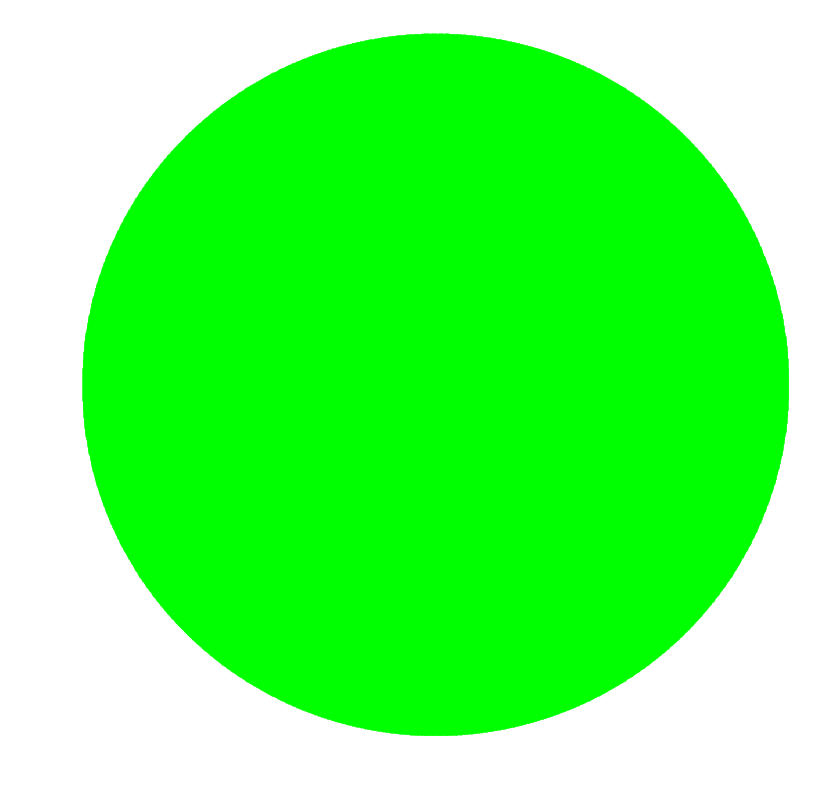
\includegraphics[width=\linewidth]{cell_to_cell_photos/celltocell0.png}
        \caption{Day 0}
    \end{subfigure}
    \begin{subfigure}[b]{0.4\linewidth}
        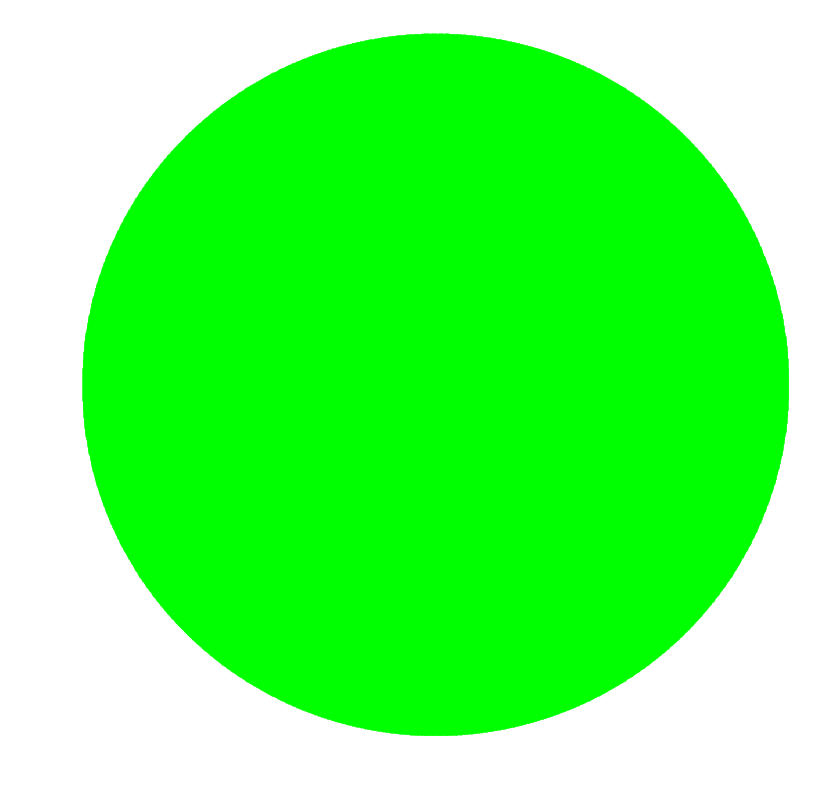
\includegraphics[width=\linewidth]{cell_free_photos/cellfree0.png}
        \caption{Day 0}
    \end{subfigure}

    \begin{subfigure}[b]{0.4\linewidth}
        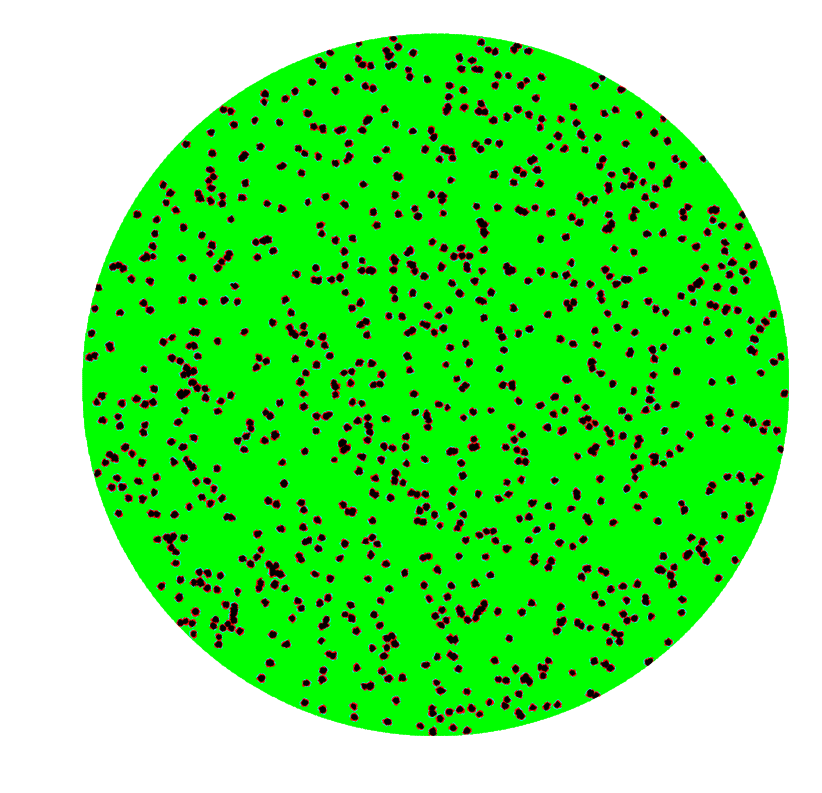
\includegraphics[width=\linewidth]{cell_to_cell_photos/celltocell1.png}
        \caption{Day 2}
    \end{subfigure}
    \begin{subfigure}[b]{0.4\linewidth}
        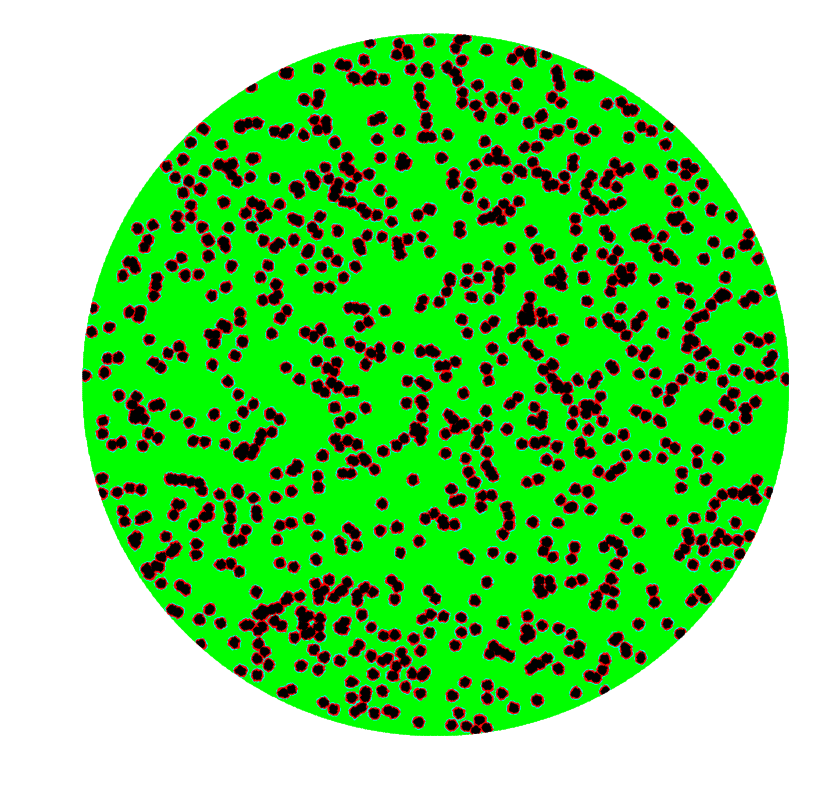
\includegraphics[width=\linewidth]{cell_free_photos/cellfree1.png}
        \caption{Day 2}
    \end{subfigure}
    
    \begin{subfigure}[b]{0.4\linewidth}
        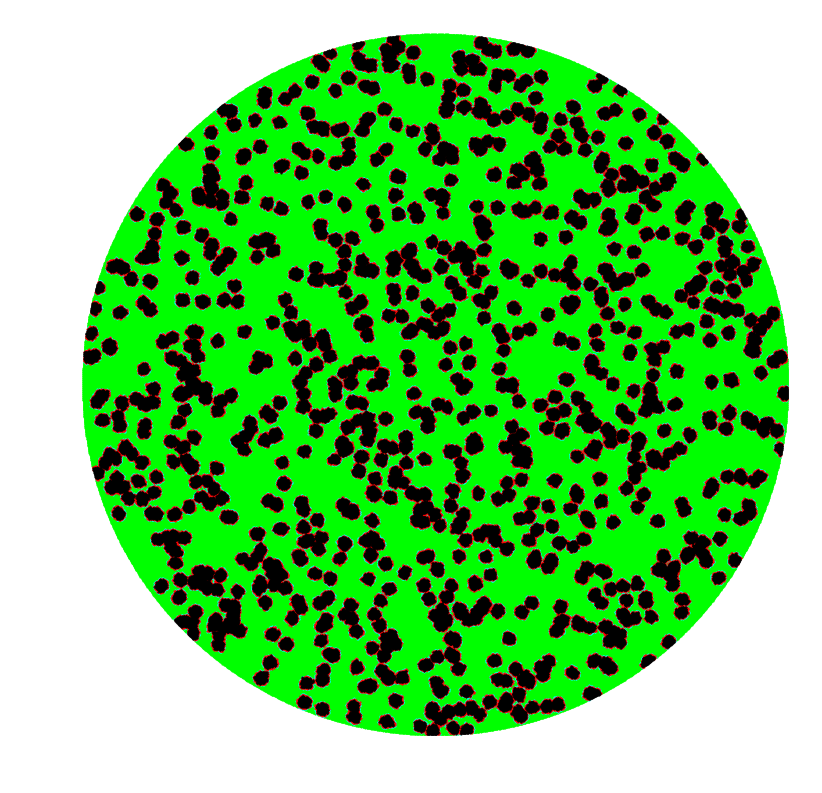
\includegraphics[width=\linewidth]{cell_to_cell_photos/celltocell2.png}
        \caption{Day 4}
    \end{subfigure}
    \begin{subfigure}[b]{0.4\linewidth}
        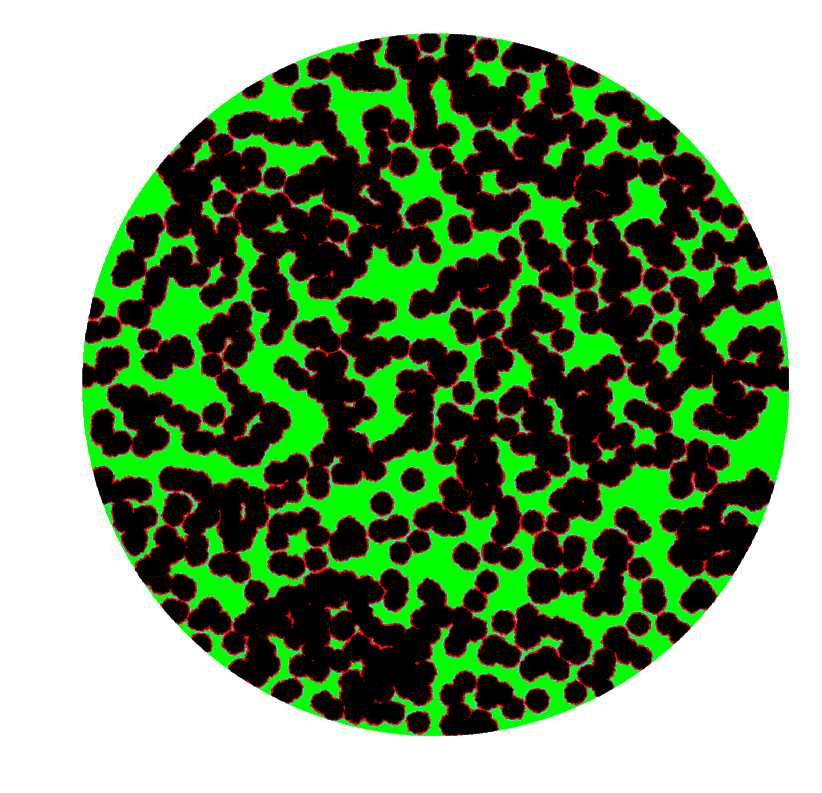
\includegraphics[width=\linewidth]{cell_free_photos/cellfree2.png}
        \caption{Day 4}
    \end{subfigure}
    
    \begin{subfigure}[b]{0.4\linewidth}
        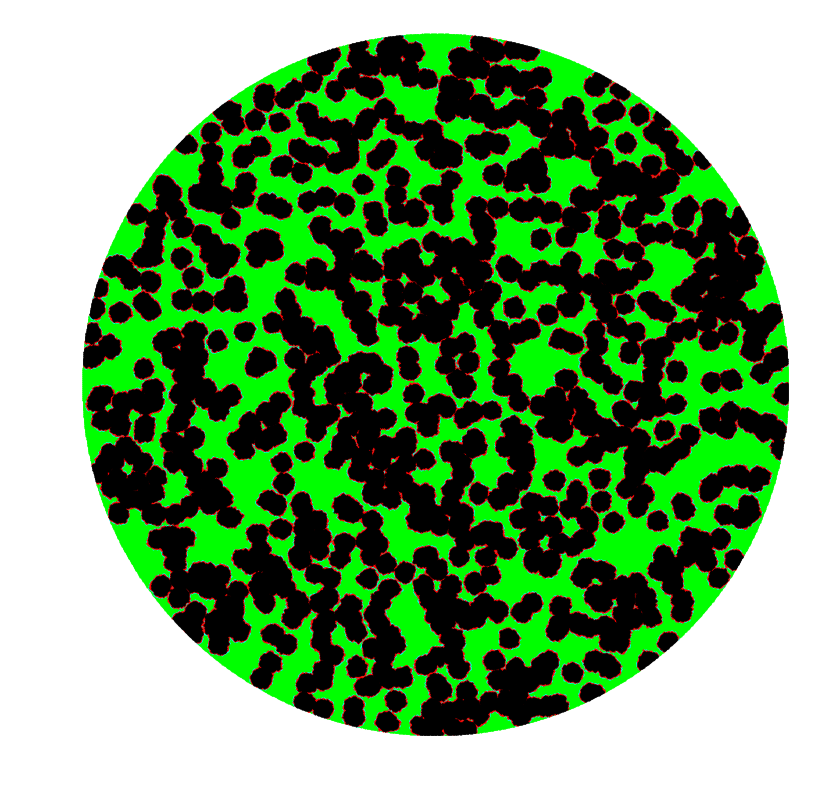
\includegraphics[width=\linewidth]{cell_to_cell_photos/celltocell3.png}
        \caption{Day 6}
    \end{subfigure}
    \begin{subfigure}[b]{0.4\linewidth}
        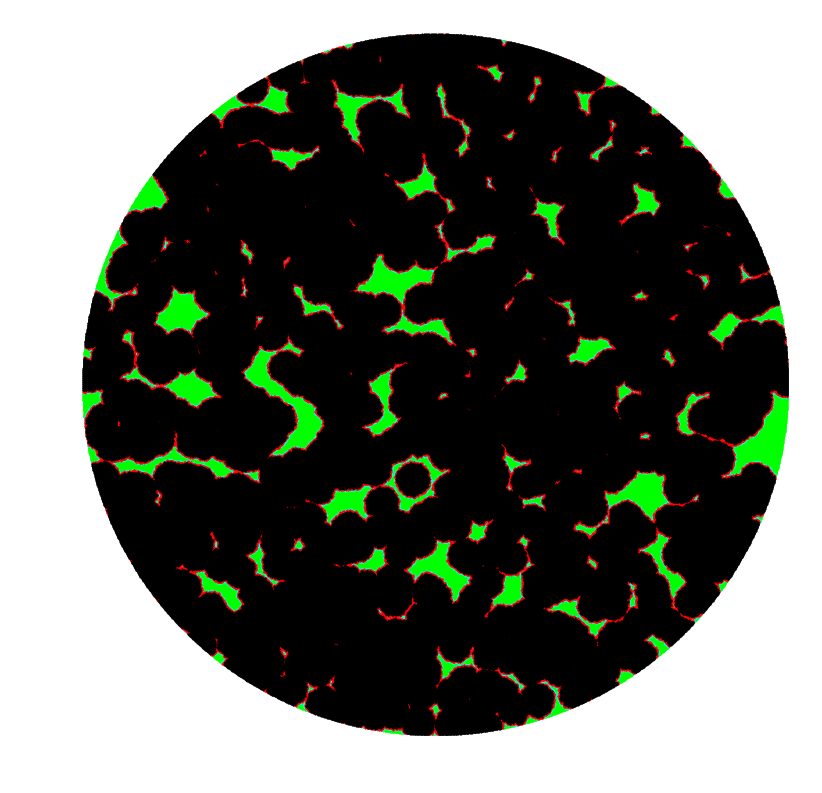
\includegraphics[width=\linewidth]{cell_free_photos/cellfree3.png}
        \caption{Day 6}
    \end{subfigure}
    
    \begin{subfigure}[b]{0.4\linewidth}
        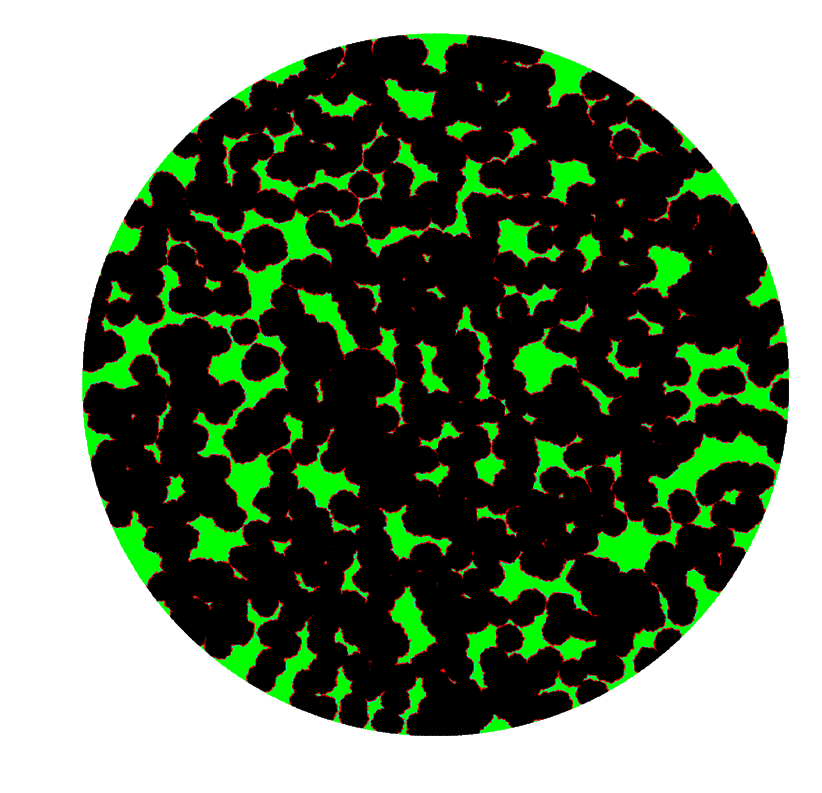
\includegraphics[width=\linewidth]{cell_to_cell_photos/celltocell4.png}
        \caption{Day 8}
    \end{subfigure}
    \begin{subfigure}[b]{0.4\linewidth}
        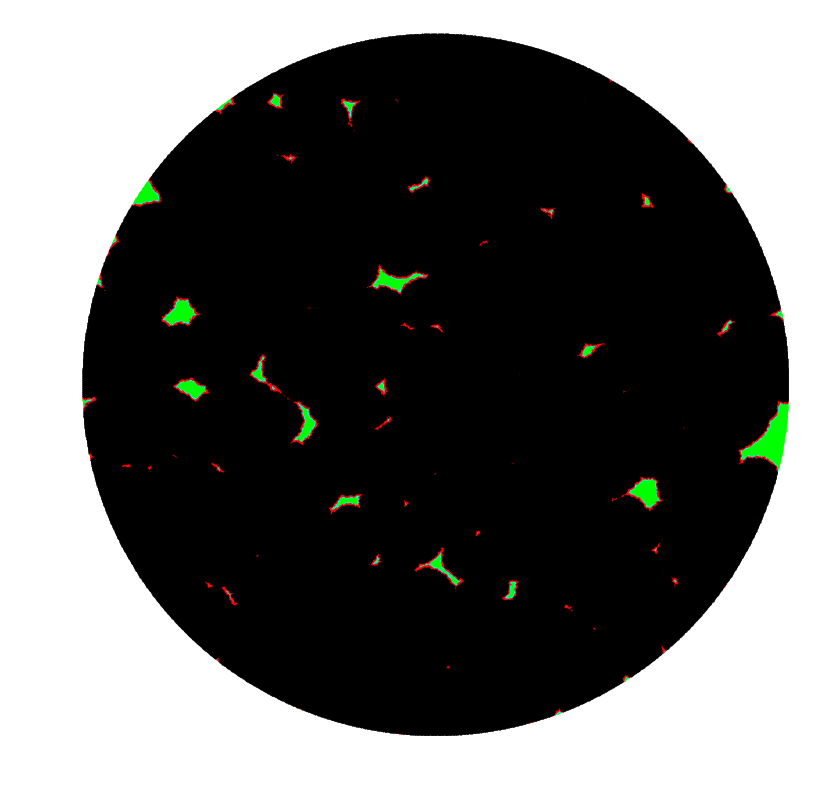
\includegraphics[width=\linewidth]{cell_free_photos/cellfree4.png}
        \caption{Day 8}
    \end{subfigure}
    \caption{Simulations of (Left) cell to cell transmission and (Right) cell free transmission in a dish containing $10^{6}$ cells.}
    \label{fig:celltocell}
\end{figure}
\end{minipage}
\end{center}

\todo{You need to start thinking of explanations for why we see these results. Why is c2c slower (later $t_p$) and why does that difference disappear at high MOI. Include these explanations in this section.}%

\subsection{Methods}
Using the model, 500 simulations per transmission mode were produced for a range of MOI's: $10^{0}$, $10^{-1}$, $10^{-2}$, $10^{-3}$, $10^{-4}$, $10^{-5}$, $10^{-6}$. The parameters for the simulations were chosen to model influenza \cite{Beauchemin} and are given in Table \ref{tab:parameters}.

\begin{table}[h]
    \centering
    \caption{The set of fixed parameters used in the simulations.}
    \begin{tabular}{|c|c|}
        \hline
        production rate of virus ($\rho$)  & $562800$ /hour\\
        \hline
        infection rate of virus ($\beta$) & $2.0$ /hour\\
        \hline
        diffusion coefficient of virus ($D$) & $6*10^{-12}$ $\mathrm{m}^2$/s\\
        \hline
        clearance rate of virus ($c$) & $0.105$ /hour\\
        \hline
        cell to cell probability ($P_{c2c}$) & $0.2$\\
        \hline
        Average time of eclipse phase ($\tau_E$) & $12.0$ hour\\
        \hline
        Average time of infectious phase ($\tau_I$) & $6.0$ hour\\
        \hline
        Number of eclipse compartments ($n_e$) & $30.0$\\
        \hline
        Number of infected compartments ($n_I$) & $100.0$\\
        \hline
    \end{tabular}
    \label{tab:parameters}
\end{table}

\todo[color=red!40]{Where did the parameters come from?}

\noindent
For each of the simulations, the total amount of virus was found and plotted as a function of time. With these plots the following characteristics were measured:

\begin{itemize}
    \item \textbf{peak viral load}: The maximum amount of virus is commonly used as an indicator of the transmissibility of an infection.
    \item \textbf{time of viral peak}: This is the time between the start of the infection and the peak of the virus.
    \item \textbf{viral upslope}: Viral upslope is the exponential growth rate of the viral titer during the first ∼1 d of infection.
    \item \textbf{viral downslope}: The viral downslope is the exponential decay rate of the viral titer and for ordinary differential equation models is linked to both the lifespan of infectious cells and the clearance rate of virus.
%    \item \textbf{area under the curve (AUC)}: AUC is often used to assess the severity of an infection (Barroso et al., 2005, Hayden et al., 2000).
%    \item \textbf{infection duration}: The infection duration is defined as the duration of time the viral titer is over $10^{4}$ and is indicative of how long an infected patient might experience symptoms (Dobrovolny et al., 2010). \todo[inline, color=red!40]{In that paper, we used the symptomatic duration which is a $10^4$ threshold. $10^1$ is a typical experimental limit of detection and gives the infection duration.}%
\end{itemize}

\noindent
To test if the above characteristics are statistically independent for the two transmission modes, cell to cell and cell free, the Mann–Whitney U test was used on the two sets of data that were produced for each transmission mode during the 500 simulations.

\subsection{Results}
In figure \ref{fig:celltocell}, the two modes of transmission look similar, but it is apparent that the cell free mode spreads the infection much quicker than the cell to cell transmission. As seen in figure \ref{fig:VirusVsTime}, the cell free viral titer curve terminates several hundred hours before the cell to cell curve.

\todo[noline]{You don't need to include it in the paper, but you should check how the viral curve as C2C probability changes.}

\begin{figure}[h]
    \centering
    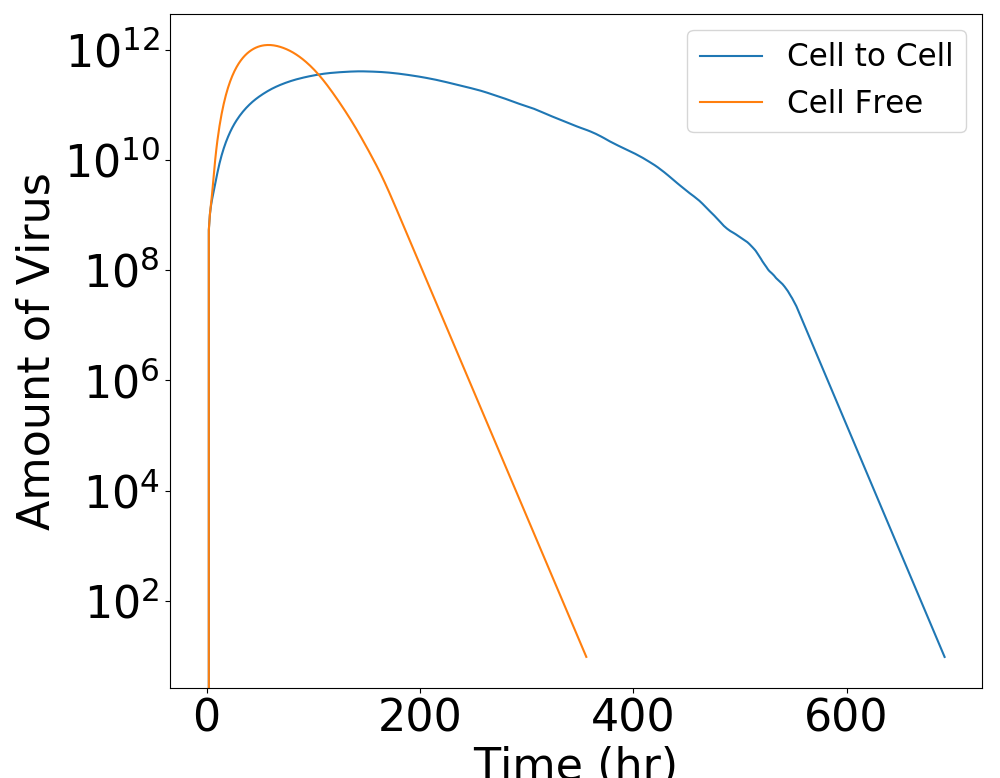
\includegraphics[width=0.8\linewidth]{Figures/VirusVsTime.png}
    \caption{A viral titer curve of a single simulation for both cell to cell and cell free transmission with MOI of $10^{-3}$ and parameters as given in Table \ref{tab:parameters}.}
    \label{fig:VirusVsTime}
\end{figure}

\begin{figure}[h]
    \centering
    \begin{subfigure}[b]{0.4\linewidth}
        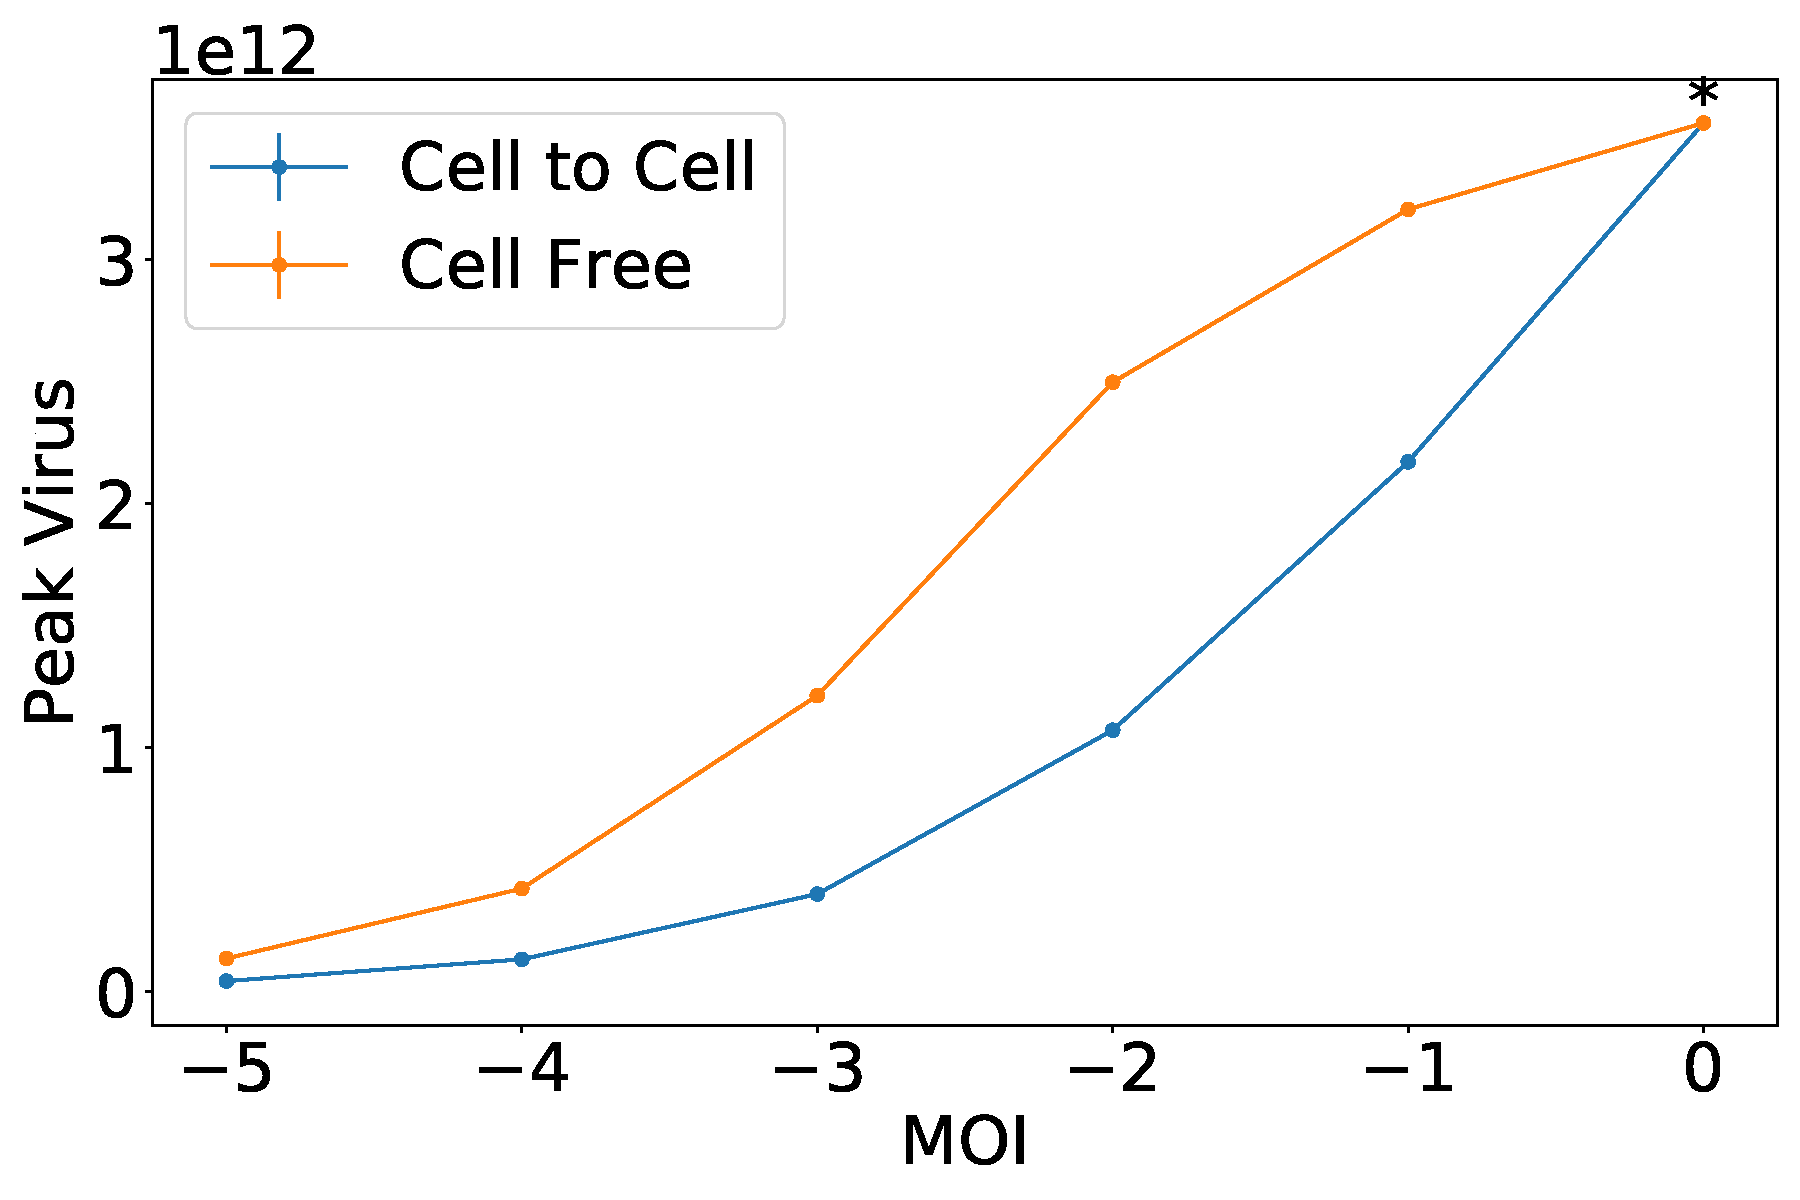
\includegraphics[width=\linewidth]{Graphs/PeakViralTittervsMOI.pdf}
        \caption{}
        \label{fig:Peak_virus_of_both_transmission_modes}
    \end{subfigure}
    \begin{subfigure}[b]{0.4\linewidth}
        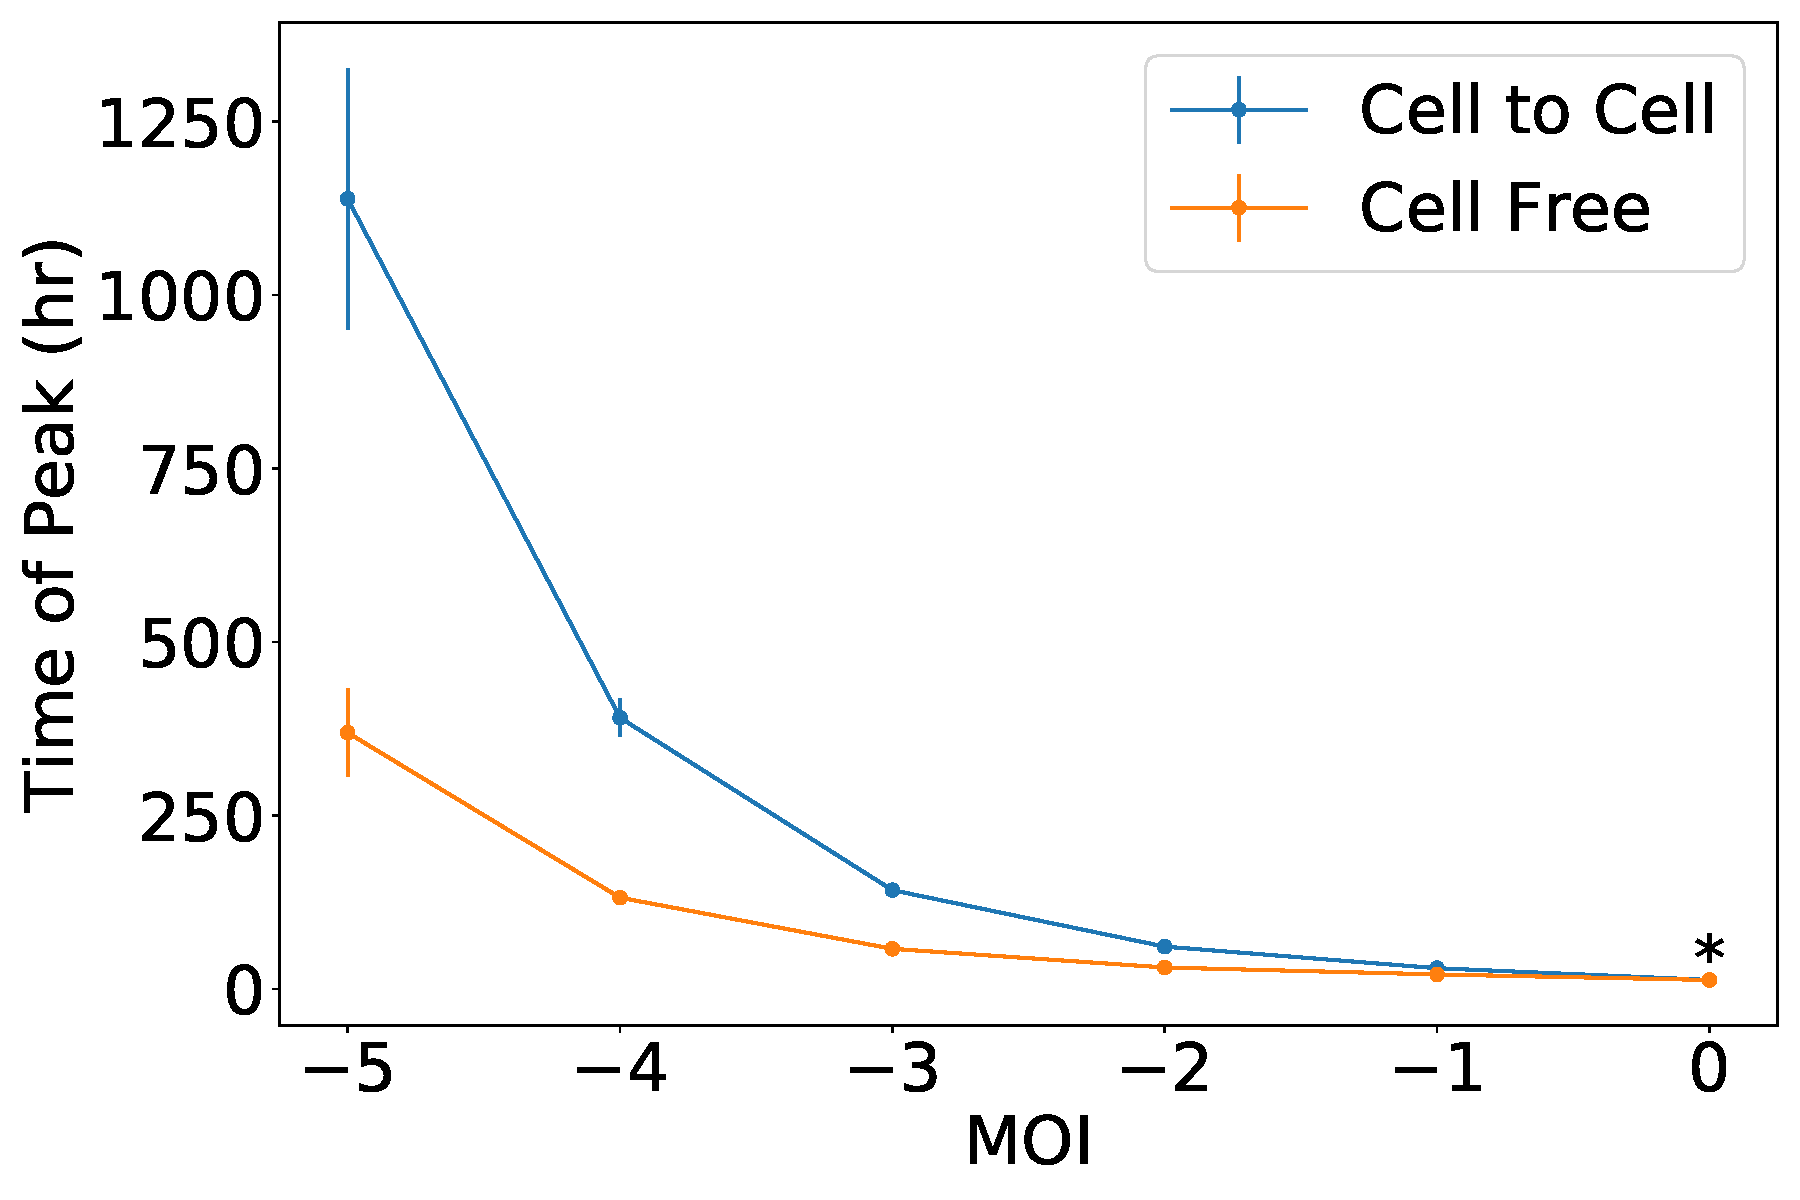
\includegraphics[width=\linewidth]{Graphs/PeakViralTitterTimevsMOI.pdf}
        \caption{}
        \label{fig:Peak_time_of_both_transmission_modes}
    \end{subfigure}
    \begin{subfigure}[b]{0.4\linewidth}
        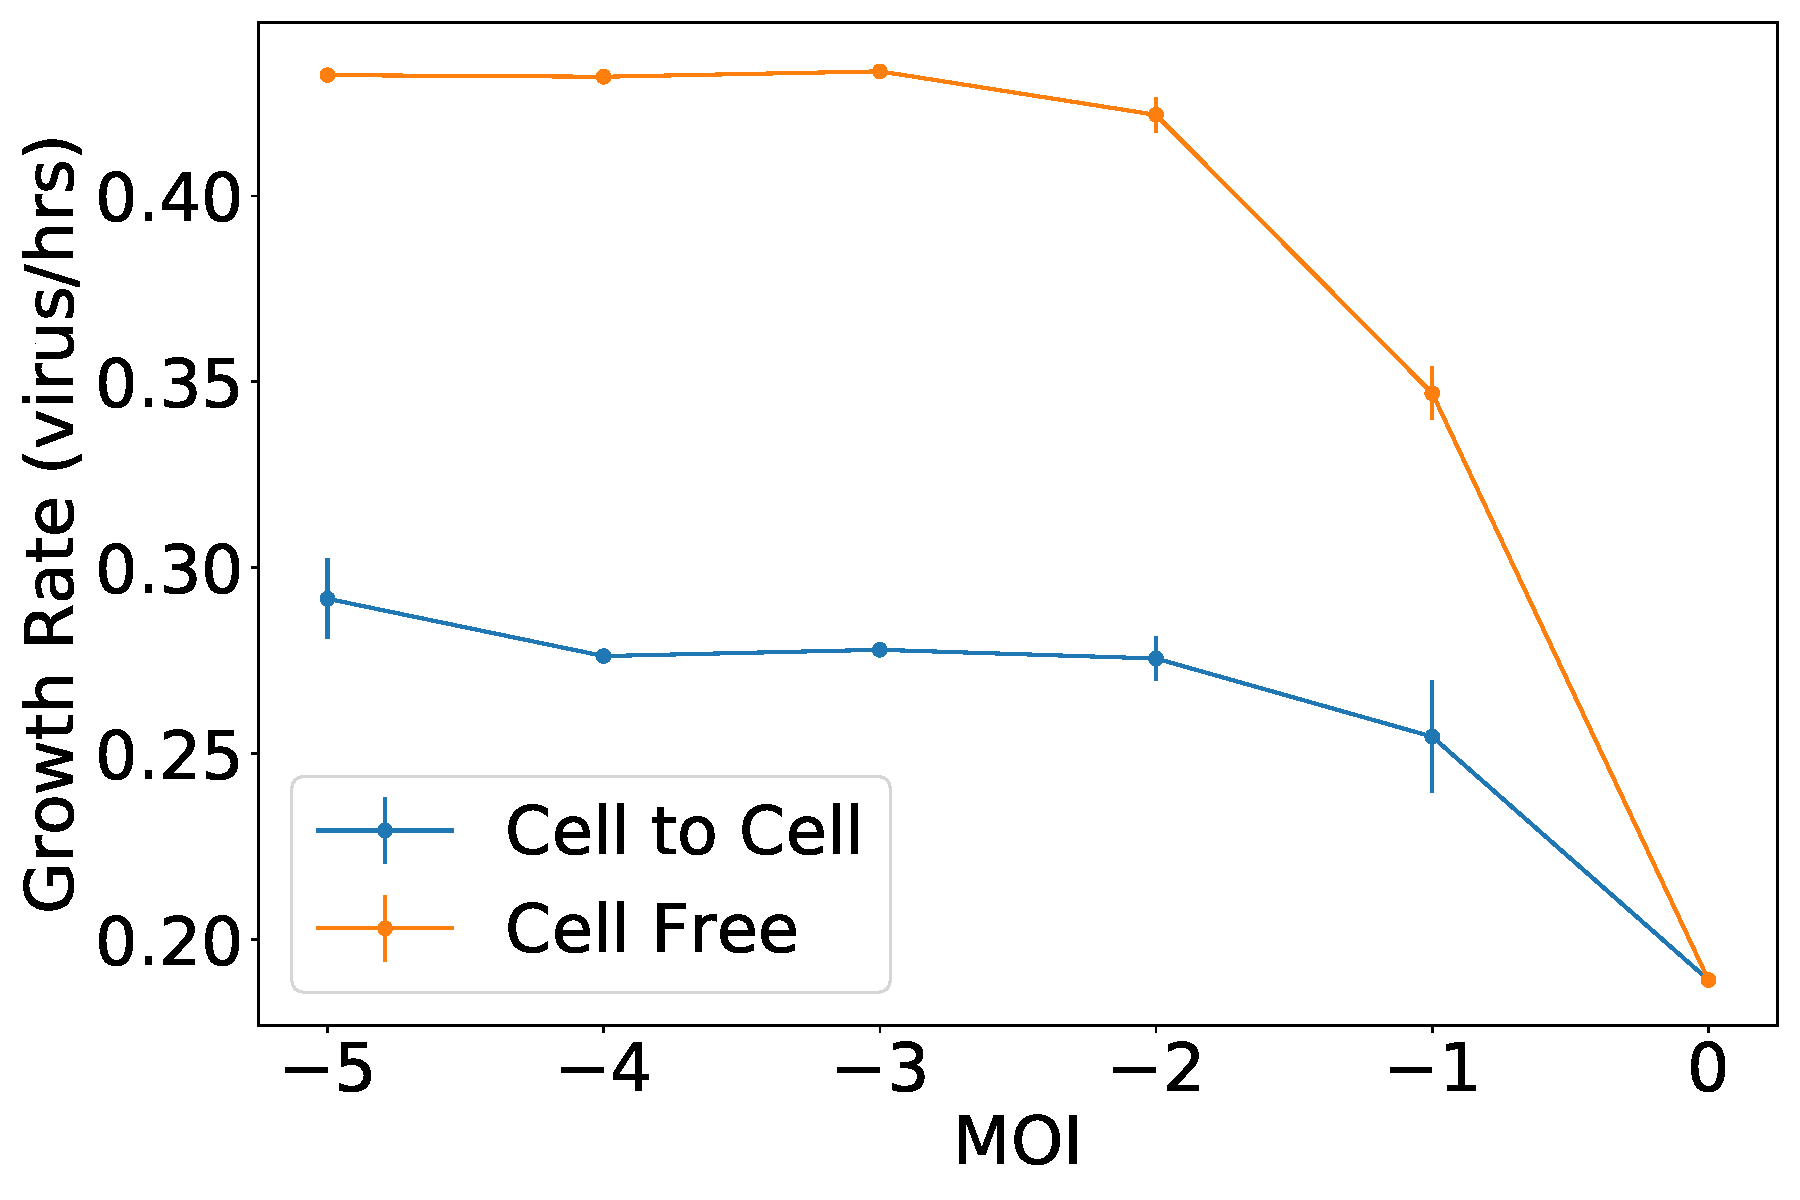
\includegraphics[width=\linewidth]{Graphs/UpSlopevsMOI.pdf}
        \caption{}
        \label{fig:Growth_Rate_of_both_transmission_modes}
    \end{subfigure}
    \begin{subfigure}[b]{0.4\linewidth}
        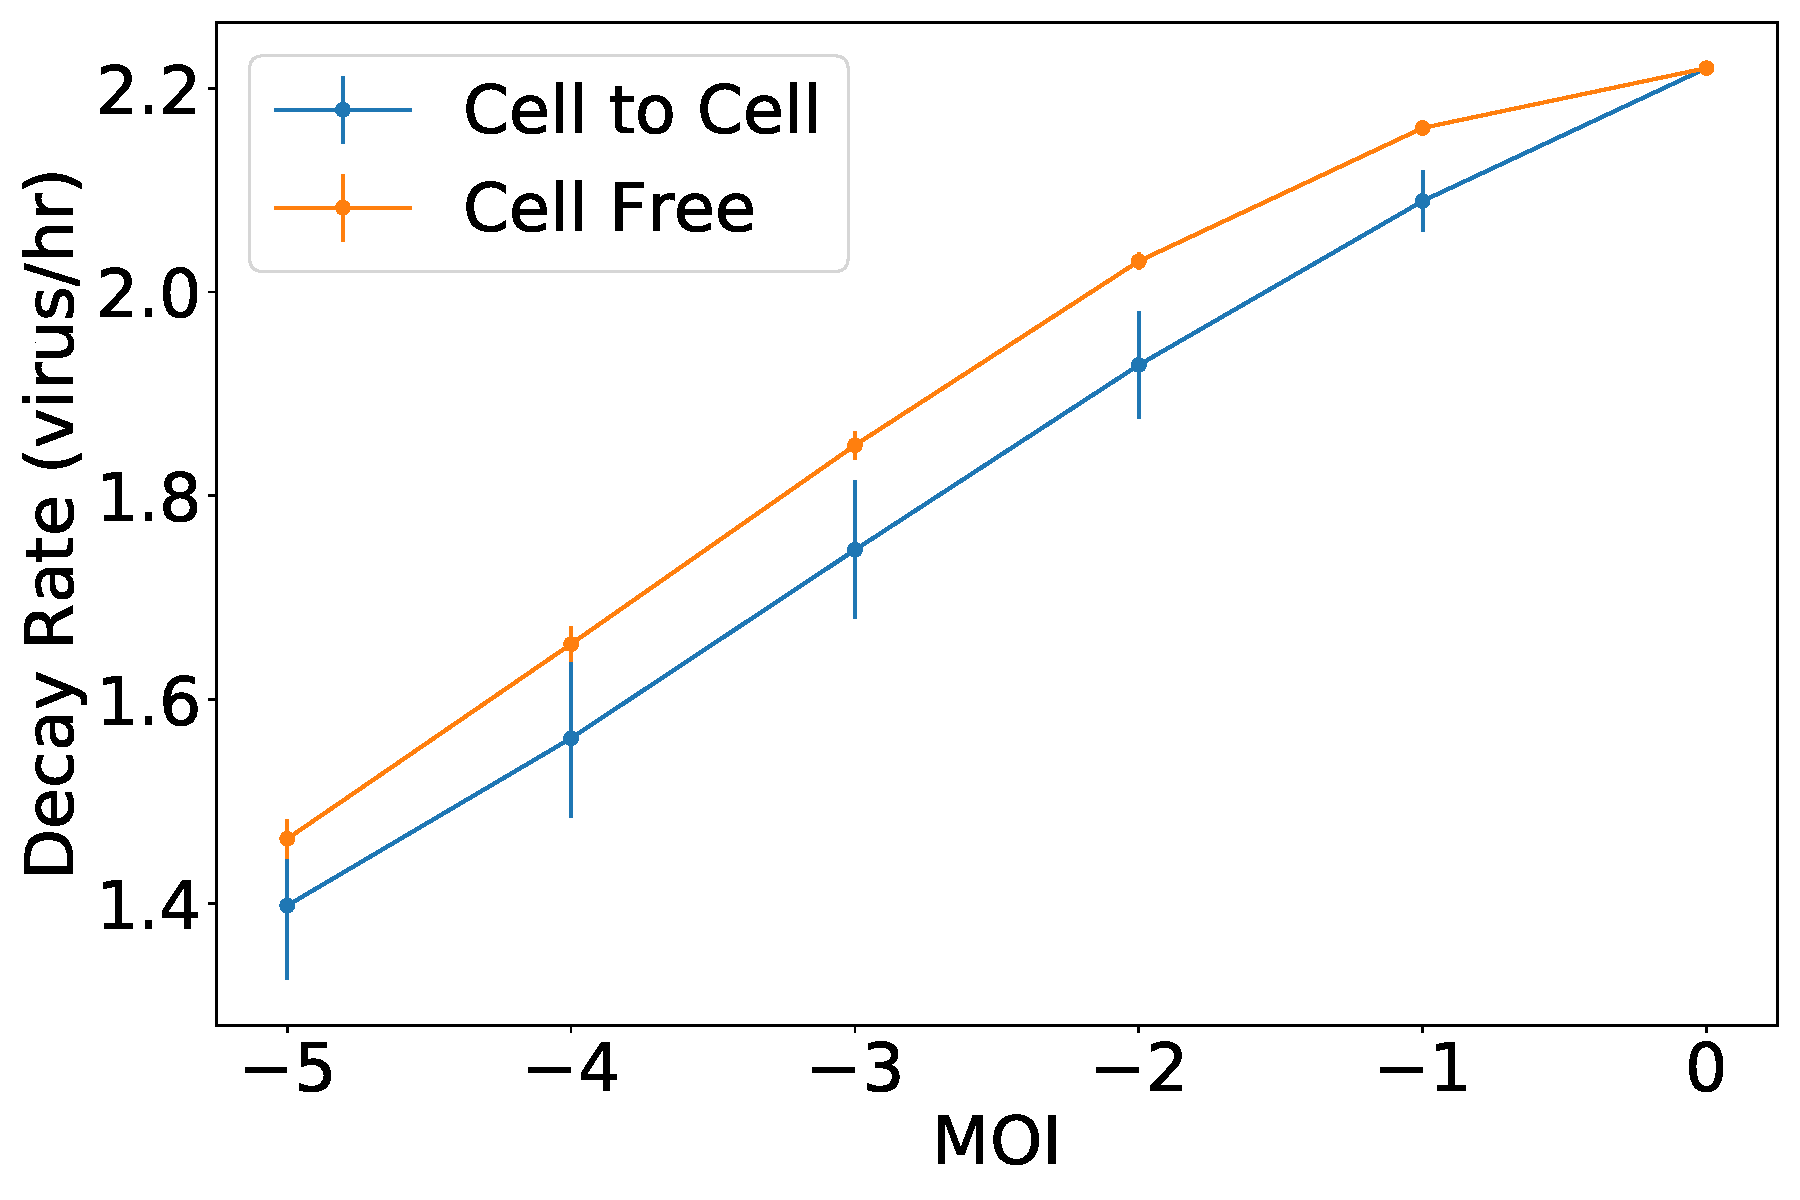
\includegraphics[width=\linewidth]{Graphs/DownSlopevsMOI.pdf}
        \caption{}
        \label{fig:Decay_Rate_of_both_transmission_modes}
    \end{subfigure}
    \caption{Viral titer characteristics for both transmission modes. For each plot the error bars show one standard deviation. a) Peak virus of vs MOI, b) Peak time vs MOI, c) Growth Rate vs MOI, d) Decay Rate vs MOI. (*) The cell to cell and cell free transmission data distributions that are not statistically independent of each other.}
    \label{fig:Graphs}
\end{figure}

Figure \ref{fig:Graphs} shows the average of the 500 simulations for each of the characteristics mentioned above plotted against each of the MOI. The error bars are one standard deviation of the 500 simulations. Figure \ref{fig:Peak_virus_of_both_transmission_modes} shows that with MOI less than one, the peak viral titer is always greater for cell free transmission with no overlapping error bars. Figure \ref{fig:Peak_time_of_both_transmission_modes} shows that with MOI less than one, the amount of time it takes for cell to cell transmission to reach the peak amount of virus is more than the cell free transmission mode with no overlapping error bars. Figure \ref{fig:Growth_Rate_of_both_transmission_modes} shows that with MOI less than one, the growth rate of the cell free transmission is always greater than the cell to cell transmission with no overlapping error bars. Figure \ref{fig:Decay_Rate_of_both_transmission_modes} shows that with MOI less than one, the decay rate is always greater for cell free transmission with no overlapping error bars. 

Using the Mann–Whitney U test, all of the characteristics for cell to cell and cell free transmission were statistically independent for a given MOI, except for peak virus and time of teak at an MOI of $10^0$. This shows that all other characteristics are identifiable and can be used to differentiate cell to cell versus cell free transmission.

\todo[noline, color=red!40]{You need to do a better job introducing and describing the figures. Remember that most of the readers do not know ANYTHING about what you're doing.}

\todo[inline, color=red!40]{Do you have the statistics results yet? What do your results tell us about the differences in how the virus spreads with the different modes?}%

\subsection{Discussion}
We found statistical significance between the two modes of transmission for the upslope, the downslope, and the peak virus and the time of peak virus where MOI is less then $10^0$. This statistical significance means that an experimentalist could measure values of peak virus at a certain MOI and be able to tell whether the virus uses only cell free or only cell to cell transmission. It is important to note that these results were generated with a fixed value of cell to cell transmission probability and they may change with different probabilities. The next phase of this work will investigate how different probabilities of cell to cell transmission  will affect the upslope, the downslope, the peak virus and the time of peak virus.

As we have shown above, it is possible to differentiate between the cell to cell and cell free transmission in the simulated infections. But the simulated data has an error that is much smaller than experimental data, table \ref{tab:AdvectionSpeeds} shows some typical experimental errors \cite{Parra, LaBarre}. Experimental viral load data is known to only be accurate to $0.5$ $\mathrm{log}_{10}$ \cite{LaBarre}, so in practice it might be difficult to tell how viruses are transmitting in certain cases.

\begin{table}[h]
    \centering
    \caption{List of typical experimental errors.}
    \begin{tabular}{|c|c|}
        \hline
        peak viral load  & $0.5$ $\mathrm{log}_{10}$ $\mathrm{TCID}_{10}$/ml\\
        \hline
        time of peak  & 0.2 d\\
        \hline
        upslope  & 0.6 /d\\
        \hline
        downslope  & 0.5 /d\\
        \hline
    \end{tabular}
    \label{tab:AdvectionSpeeds}
\end{table}

\clearpage

\section{References Cited}
%\textcolor{blue}{
%All references (background, techniques, methods, etc.) using in the proposal must be cited properly. See http://journals.aas.org/authors/references.html for formatting of Astronomy-based research and for Physics/Bio-Physics-based see: https://publishing.aip.org/authors/preparing-your-manuscript.}



\begin{thebibliography}{9}
%\bibitem{Dict} 
%"virus." 
%\textit{Merriam-Webster.com}. 2020. 
%https://www.merriam-webster.com (18 Jan 2020).

\bibitem{website2}
Vidyasagar, Aparna. 
“What Are Viruses?”
\textit{Live Science}, 
Live Science Contributor, 6 Jan 2016, 
\url{https://www.livescience.com/53272-what-is-a-virus.html}.

\bibitem{Allen} 
Linda J.S. Allen, Elissa J. Schwartz. 
\textit{Free-virus and cell-to-cell transmission in models of equine infectious
anemia virus infection}. 
Mathematical Biosciences, 2015.

\bibitem{website1} 
"Useful Numbers for Cell Culture",
\\
\texttt{\url{https://www.thermofisher.com/us/en/home/references/gibco-cell-culture-basics/cell-culture-protocols/cell-culture-useful-numbers.html}}

\bibitem{Bruckner} 
Bastian R. Br{\"u}ckner, Andreas Janshoff.
\textit{Importance of integrity of cell-cell junctions for the mechanics of confluent MDCK II cells}. 
Scientific Reports, 2018.

\bibitem{Holder} 
Benjamin P. Holder, Laura E. Liao, Philippe Simon, Guy Boivin, and Catherine A. A. Beauchemin
\textit{Design considerations in building in silico equivalents of common
experimental influenza virus assays}. 
Informa, 2011.

\bibitem{Kumar}
Kumar, Panka
"Virus Identification and Quantification"
\textit{MATER METHODS} 2013;3:207
//dx.doi.org/10.13070/mm.en.3.207

\bibitem{Kaiser}
Gary Kaiser, Erica Suchman. 
2008. 
Productive life cycle of animal viruses animations. 

\bibitem{website3} 
"Lecture 2: Virus Structure",
\\
\texttt{\url{https://msu.edu/course/mmg/569/Virus\%20Structure.html}}

\bibitem{website4}
"This Past Flu Season Was the Longest in 10 Years, the CDC Says",
\\
\texttt{\url{https://time.com/5610878/2018-2019-flu-season/}}

\bibitem{RespiratoryTract}
"Illu\_conducting\_passages",
Lord Akryl, Jmarchn
\\
\texttt{\url{http://cancer.gov, Public Domain, https://commons.wikimedia.org/w/index.php?curid=10296586}}

\bibitem{cell2cell} 
Amrita Kumar, Jin Hyang Kim, Priya Ranjan, Maureen G. Metcalfe, Weiping Cao,
Margarita Mishina, Shivaprakash Gangappa, Zhu Guo, Edward S. Boyden, Sherif Zaki,
Ian York, Adolfo García-Sastre, Michael Shaw \& Suryaprakash Sambhara
\textit{Influenza virus exploits tunneling nanotubes for cell-to-cell spread}. 
Scientific Reports, 2017.

\bibitem{Smith} 
Amber M. Smith, Frederick R. Adler, Julie L. McAuley, Ryan N. Gutenkunst, Ruy M. Ribeiro, Jonathan A. McCullers, Alan S. Perelson
\textit{Effect of 1918 PB1-F2 Expression on Influenza A Virus Infection Kinetics}. 
PLOS Computational Biology, 2011.

\bibitem{bacacam06} 
Prasith Baccam, Catherine Beauchemin, Catherine A. Macken, Frederick G. Hayden, and Alan S. Perelson
\textit{Kinetics of Influenza A Virus Infection in Humans}. 
Journal of Virology, 2006.

\bibitem{diffusionmodel} 
Gilberto González-Parra, Hana M. Dobrovolny
\textit{The rate of viral transfer between upper and lower
respiratory tracts determines RSV illness duration}. 
Journal of Mathematical Biology, 2019.

\bibitem{plosRSV} 
Gilberto Gonzàlez-Parra, Filip De Ridder, Dymphy Huntjens, Dirk Roymans, Gabriela Ispas, Hana M. Dobrovolny
\textit{A comparison of RSV and influenza in vitro kinetic
parameters reveals differences in infecting time}. 
PLOS One, 2018.

\bibitem{Quirouette} 
Christian Quirouette, Nada P. Younis, Micaela B. Reddy, Catherine A.A. Beauchemin
\textit{A mathematical model describing the localization and spread of
influenza A virus infection within the human respiratory tract}. 
arXiv, 2019.

\bibitem{Geoghegan}
Geoghegan S, Erviti A, Caballero MT, Vallone F, Zanone SM, Ves Losada J, Bianchi A, Acosta PL, Talarico LB, Ferretti A, Alva Grimaldi L, Sancilio A, Duenas K, Sastre G, Rodriguez A, Ferrero F, Barboza E, Gago GF, Nocito C, Flamenco E, Perez AR, Rebec B, Ferolla FM, Libster R, Karron RA, Bergel E, Polack FP
\textit{Mortality due to respiratory syncytial virus burden and risk factors}. 
American Journal of Respiratory and Critical Care Medicine, 2017.

\bibitem{Fleming}
Fleming DM, Taylor RJ, Lustig RL, Schuck-Paim C, Haguinet F, Webb DJ, Logie J, Matias G, Taylor S
\textit{Modelling estimates of the burden of respiratory syncytial virus infection in adults and the elderly in the united kingdom}.
BMC Infectious Diseases, 2015.

\bibitem{Hall}
Hall C, Long C, Schnabel K
\textit{Respiratory syncytial virus infections in previously healthy working
adults}. 
Clinical Infectious Diseases, 2001.

\bibitem{Lee}
Lee FEH, Walsh EE, Falsey AR, Betts RF, Treanor JJ
\textit{Experimental infection of humans with A2
respiratory syncytial virus}. 
Antiviral Research, 2004.

\bibitem{Bagga}
Bagga B, Woods CW, Veldman TH, Gilbert A, Mann A, Balaratnam G, Lambkin-Williams R, Oxford JS, McClain MT, Wilkinson T, Nicholson BP, Ginsburg GS, DeVincenzo JP (2013) 
\textit{Comparing influenza and RSV viral disease dynamics in experimentally infected adults predicts clinical effectiveness of RSV antivirals}. 
Antiviral Therapy, 2013

\bibitem{Mills}
Mills J, Vankirk J, Wright P, Chanock R
\textit{Experimental respiratory syncytial virus infection of adults—possible mechanisms of resistance to infection and illness}. 
Journal Immunology, 1971.

\bibitem{Naorat}
Naorat S, Chittaganpitch M, Thamthitiwat S, Henchaichon S, Sawatwong P, Srisaengchai P, Lu Y, Chuananon S, Amornintapichet T, Chantra S, Erdman DD, Maloney SA, Akarasewi P, Baggett HC
\textit{Hospitalizations for acute lower respiratory tract infection due to respiratory syncytial virus in thailand, 2008–2011}.
The Journal of Infectious Diseases, 2013

\bibitem{Kaneko}
Kaneko M, Watanabe J, Ueno E, Hida M, Sone T (2001) 
\textit{Risk factors for severe respiratory syncytial virus-associated lower respiratory tract infection in children}.
Pediatrics International, 2001.

\bibitem{Shi}
Shi T, Balsells E, Wastnedge E, Singleton R, Rasmussen Z, Zar HJ, Rath BA, Madhi SA, Campbell S, Vaccari LC, Bulkow LR, Thomas ED, Barnett W, Hoppe C, Campbell H, Nair H
\textit{Risk factors for respiratory syncytial virus associated with acute lower respiratory infection in children under five years: systematic review and meta-analysis}. 
Journal of Global Health, 2015.

\bibitem{Atwell}
Atwell JE, Geoghegan S, Karron RA, Polack FP
\textit{Clinical predictors of critical lower respiratory
tract illness due to respiratory syncytial virus in infants and children: data to inform case definitions for efficacy trials}. 
The Journal of Infectious Diseases, 2016

\bibitem{HallC}
Hall C, Long C, Schnabel K 
\textit{Respiratory syncytial virus infections in previously healthy working
adults}.
Clinical Infectious Diseases, 2001.

\bibitem{Takeyama}
Takeyama A, Hashimoto K, Sato M, Kawashima R, Kawasaki Y, Hosoya M
\textit{Respiratory syncytial virus shedding by children hospitalized with lower respiratory tract infection}. 
Journal Medical Virology, 2016.

\bibitem{Park}
Park SY, Kim T, Jang YR, Kim MC, Chong YP, Lee SO, Choi SH, Kim YS, Woo JH, Kim SH
\textit{Factors predicting life-threatening infections with respiratory syncytial virus in adult patients}.
Infectious Diseases, 2017.

\bibitem{Gallagher}
Molly E. Gallagher, Christopher B. Brooke, Ruian Ke, and Katia Koelle
\textit{Causes and Consequences of Spatial Within-Host Viral Spread}.
Viruses, 2018.

\bibitem{Pourbashash}
Hossein Pourbashash, Sergei S. Pilyugin and Patrick De Leenheer
\textit{Global Analysis of within Host Virus Models with Cell-to-Cell Viral Transmission}.
Discrete \& Continuous Dynamical Systems, 2014.

\bibitem{Wang}
Xia Wang, Libin Rong
\textit{HIV low viral load persistence under treatment: Insights from a model of cell-to-cell viral transmission}.
Applied Mathematics Letters, 2019.

\bibitem{Sturm}
Sturm R
\textit{Theoretical models of carcinogenic particle deposition and clearance in children’s lungs}.
Journal of Thoracic Disease, 2012.

\bibitem{Puchelle}
Puchelle E, Zahm J, Bertrand A
\textit{Influence of age on bronchial mucociliary transport}.
Scandinavian Journal of Respiratory Diseases, 1979

\bibitem{Grubb}
Grubb BR, Livraghi-Butrico A, Rogers TD, Yin W, Button B, Ostrowski LE
\textit{Prophylactic administration of respiratory syncytial virus immune globulin to high-risk infants and young children}. 
American Journal of Physiology, 2016.

\bibitem{Oliveira}
de Oliveira-Maul JP, de Carvalho HB, Goto DM, Maia RM, Flo C, Barnabe V, Franco DR, Benabou S, Perracini MR, Jacob-Filho W, Saldiva PHN, Lorenzi-Filho G, Rubin BK, Nakagawa NK
\textit{Aging, diabetes, and hypertension are associated with decreased nasal mucociliary clearance}.
Chest, 2013

\bibitem{Ho}
Ho J, Chan K, Hu W, Lam W, Zheng L, Tipoe G, Sun J, Leung R, Tsang K
\textit{The effect of aging on nasal mucociliary clearance, beat frequency, and ultrastructure of respiratory cilia}. 
American Journal of Respiratory and Critical Care Medicine, 2001.

\bibitem{Li}
Yan Li, Andreas Handel
\textit{Modeling inoculum dose dependent patterns of acute virus infections}
Journal of Theoretical Biology, 2014

\bibitem{Moore}
James R. Moore, Hasan Ahmed, Balaji Manicassamy, Adolfo Garcia-Sastre, Andreas Handel \& Rustom Antia
\textit{Varying Inoculum Dose to Assess the Roles of the Immune Response and Target Cell Depletion by the Pathogen in Control of Acute Viral Infections}.
Bulletin of Mathematical Biology, 2020

\bibitem{Beauchemin}
Catherine Beauchemin, John Samuel, Jack Tuszynski
\textit{A simple cellular automaton model for influenza A viral infections}.
Journal of Theoretical Biology, 2005

\bibitem{LaBarre}
David D. LaBarre, R. Joel Lowy
\textit{Improvements in methods for calculating virus titer estimates from TCID 50 and plaque assays}.
Journal of Virological Methods, 2001.

\bibitem{Carmichael}
Carmichael JC, Yokota H, Craven RC, Schmitt A, Wills JW.
\textit{The HSV-1 mechanisms of cell-to-cell spread and fusion are critically dependent on host PTP1B}.
PLoS Pathogens, 2018.

\bibitem{Chowdhury}
Chowdhury MI, Koyanagi Y, Suzuki M, Kobayashi S, Yamaguchi K, Yamamoto N.
\textit{Increased production of human immunodeficiency virus (HIV) in HIV-induced syncytia formation: an efficient infection process}.
Virus Genes, 1992.

\bibitem{Rozieres}
Aurore Rozières, Christophe Viret, and Mathias Faure
\textit{Autophagy in Measles Virus Infection}.
Viruses, 2017.

\bibitem{Tian}
Jane Tian, Kelly Huang, Subramaniam Krishnan, Catherine Svabek, Daniel C. Rowe, Yambasu Brewah, Miguel Sanjuan, Andriani C. Patera, Roland Kolbeck, Ronald Herbst, and Gary P. Sims
\textit{RAGE inhibits human respiratory syncytial virus syncytium formation by interfering with F-protein function}.
Journal of General Virology, 2013.

\bibitem{Parra}
Gilberto González-Parra, Thalia Rodriguez, Hana M. Dobrovolny
\textit{A comparison of methods for extracting influenza viral titer
characteristics}.
Journal of Virological Methods, 2016.

\end{thebibliography}

\end{document}

